\documentclass[11pt,a4paper]{article}
\usepackage[margin=1in]{geometry}
\usepackage{graphicx}
\usepackage{booktabs}
\usepackage{amsmath}
\usepackage{hyperref}
\usepackage[usenames,dvipsnames]{xcolor}
\usepackage{float}
\usepackage{caption}
\usepackage{subcaption}
\usepackage{setspace}

\hypersetup{colorlinks=true, linkcolor=NavyBlue, citecolor=NavyBlue, urlcolor=NavyBlue}
\onehalfspacing

\title{%
  Portable EEG Correlates of Basketball Free-Throw Performance:\\
  Multi-Block Session Analysis Report
}
\author{Lukas Laskowski \and Kyle E.\ Mathewson}
\date{March 15, 2026}

\begin{document}
\maketitle

% ────────────────────────────────────────────────────────────────────────────
\begin{abstract}
This report presents the analysis of a multi-block free-throw session recorded
using the FreethrowEEG system. The participant performed 3 blocks of
40 free throws each, yielding 78 analysed shots (34 made,
44 missed; 44\%) after data quality screening and exclusion
of experimenter-flagged trials. Continuous EEG band power (delta, theta, alpha,
beta, gamma) was recorded from a Muse~2 headset. Shot-locked epochs were
extracted and compared between successful and unsuccessful attempts. Video was
recorded for two of the three blocks; post-hoc pose estimation using MediaPipe
was performed on the available video to extract biomechanical features aligned
with neural dynamics. Descriptive statistics, time-series visualizations, pose
kinematics, and exploratory inferential tests are reported. Data were collected across 3 blocks of 40 shots each. After data quality screening and exclusion of experimenter-flagged trials, 78 shots were retained for EEG analysis.
\end{abstract}

% ────────────────────────────────────────────────────────────────────────────
\section{Introduction}

Electroencephalography (EEG) has been widely used to study neural correlates of
motor performance, including precision sport tasks such as archery, shooting,
and golf putting. A consistent finding in the literature is that successful
performers exhibit distinct pre-performance EEG patterns, particularly reduced
alpha desynchronization and modulated theta activity, compared to unsuccessful
attempts. This session tests whether such patterns are detectable using a
portable, four-channel Muse~2 headset during basketball free-throw shooting.

This report extends an initial pilot by using real EEG data collected over
multiple blocks, providing substantially more statistical power ($N =
$78 shots) and improved experimental control including better video
framing and consistent shot-cue logging.

The present analysis focuses on:
\begin{enumerate}
  \item Visualizing continuous and shot-locked EEG band power;
  \item Comparing pre-shot, execution, and post-shot neural signatures between
        made and missed free throws;
  \item Evaluating the theta/alpha ratio as a candidate readiness marker;
  \item Examining shot-by-shot band power progression across the session;
  \item Biomechanical pose analysis from concurrent video (where available).
\end{enumerate}

% ────────────────────────────────────────────────────────────────────────────
\section{Methods}

\subsection{Participant and Task}
The participant (Lukas) performed 3 blocks of 40 free throws
(120 total), collected in a public gymnasium on a single day. The full session
spanned approximately 51.8 minutes of active recording. Each trial
followed a structured protocol: a preparation phase ($\sim$5\,s), a pre-shot
baseline ($\sim$5\,s), shot execution ($\sim$2\,s), post-shot recording
($\sim$3\,s), and a review phase. Shot outcome (made/missed) was coded by the
participant.

\subsection{Data Quality and Exclusions}
Block~1: 3 analysed of 40 shots (0 excluded, 37 invalid EEG; with video); Block~2: 39 analysed of 40 shots (1 excluded, 0 invalid EEG; no video); Block~3: 36 analysed of 40 shots (4 excluded, 0 invalid EEG; with video). In Block~1, an EEG recording buffer issue caused the raw
data stream to stop after approximately 3 minutes, yielding valid EEG for only
the first 3 shots; the remaining 37 shots in that block had degenerate
timestamps and were excluded from analysis. The experimenter also reported
missed shot cues on certain trials: Block~1 shots 18 and 35, Block~2 shot 34,
and Block~3 shots 8, 21, 22, and 25 were excluded. After all filtering,
78 shots were retained for EEG analysis (34 made, 44
missed; 44\% accuracy).

Video was recorded for Blocks~1 and 3 but not for Block~2 (the video file did
not save). Due to the EEG timing issues in Block~1, video analysis was
performed primarily on Block~3 (36 shots).

\subsection{EEG Recording}
EEG was recorded continuously using a Muse~2 headband (four channels: TP9,
AF7, AF8, TP10; 256\,Hz sampling rate). Band power was computed in real time
using a 1-second sliding window with 25\% overlap. A 4th-order Butterworth
bandpass filter was applied to extract five standard frequency bands: delta
(1--4\,Hz), theta (4--8\,Hz), alpha (8--13\,Hz), beta (13--30\,Hz), and gamma
(30--50\,Hz). Environmental line noise was removed via a Butterworth notch
filter at 60\,Hz. For the continuous power analysis, raw electrode signals were
averaged across all four channels and band power was recomputed offline.

\subsection{Video Recording and Pose Estimation}
Video was recorded simultaneously at 30\,fps (WebM/VP9 codec) using the device
camera. Post-hoc pose estimation was performed using the MediaPipe Pose
Landmarker (heavy model), extracting 33 body landmarks per frame.
Biomechanical features---elbow angle (shoulder--elbow--wrist), wrist height,
knee angle (hip--knee--ankle), and body lean angle (torso deviation from
vertical)---were computed for each frame during the shot execution phase. Ball
release was estimated as the frame where wrist velocity peaked while the wrist
was near its highest position.

\subsection{Analysis}
Continuous EEG data were segmented into shot-locked epochs aligned to the onset
of the execution phase. Epochs were interpolated onto a common time grid
($-$12 to $+$8\,s relative to shot onset at 0.25\,s resolution) and averaged
separately for made and missed shots. Phase-wise mean power was compared using
Welch's $t$-test (unequal variances) and the Mann--Whitney $U$ test. Effect
sizes are reported as Cohen's $d$.

All 78 shots with valid EEG data across all three blocks were used for
the EEG analyses (Figures~1--8 and Table~1). Video-based analyses
(Figures~9--13) used only the subset of shots from blocks with available video.

Individual shot clips were extracted from the video, and stop-motion frame
sequences were generated for each trial. Average frame composites were created
by pixel-averaging release-point frames within each outcome group. ``Ghost''
overlays show the variability in shooting form by superimposing skeleton
renderings from all shots within a group.

% ────────────────────────────────────────────────────────────────────────────
\section{Results}

\subsection{Session Overview}
The participant completed 78 analysed shots across 3 blocks
over approximately 51.8 minutes of active recording (44\%
accuracy). Figure~\ref{fig:raster} shows the session timeline with shot phases
and outcomes overlaid on the continuous alpha power trace. Block boundaries are
indicated by vertical dashed lines.

\begin{figure}[H]
  \centering
  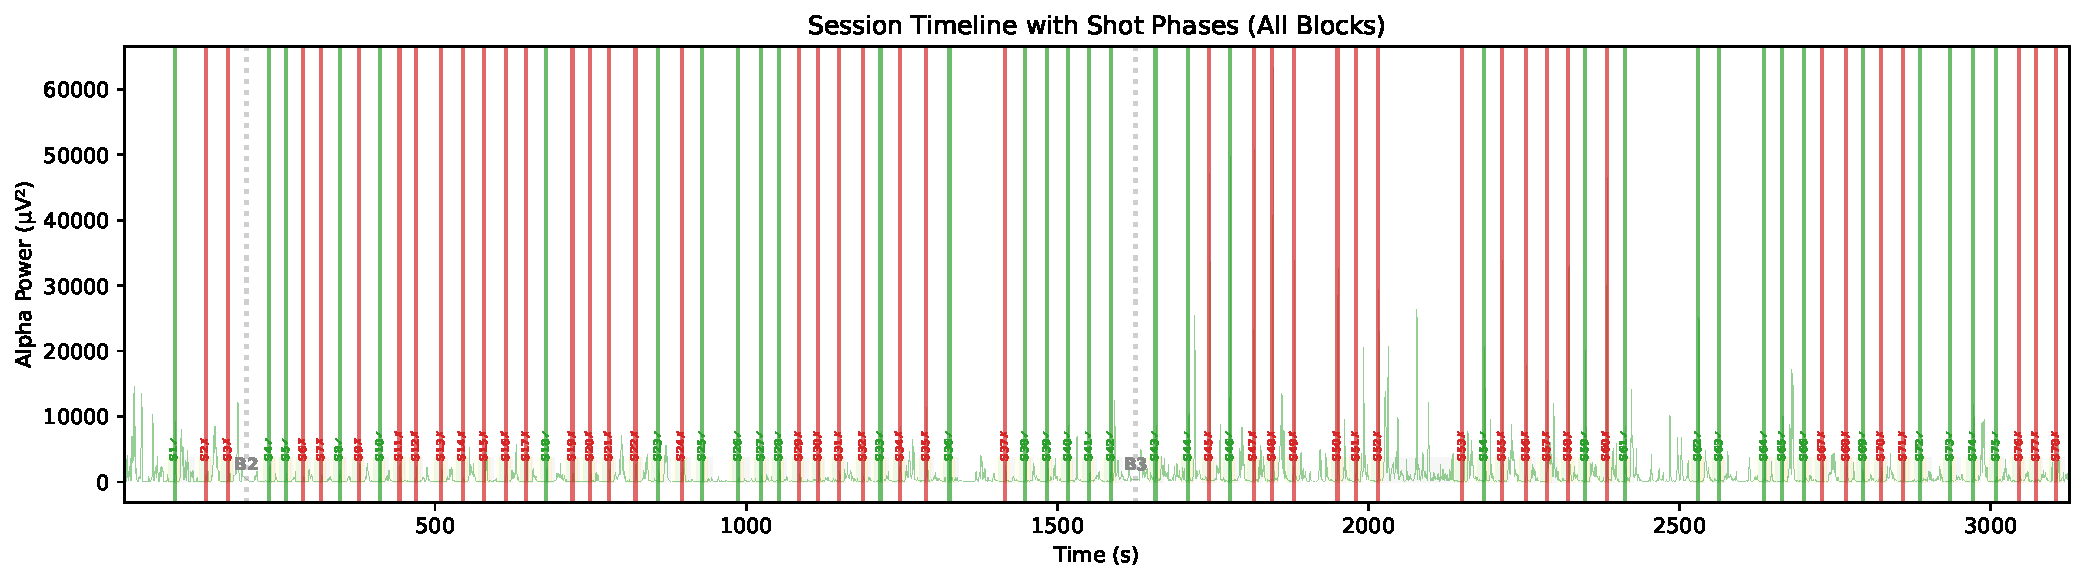
\includegraphics[width=\textwidth]{figures/fig_shot_raster.pdf}
  \caption{Session timeline. Each vertical line marks a shot (green = made,
  red = missed). Shaded regions indicate trial phases. Dotted grey lines
  mark block boundaries.}
  \label{fig:raster}
\end{figure}

\subsection{Continuous Band Power}
Figure~\ref{fig:continuous} shows the five frequency bands across all blocks.
Visual inspection of the continuous traces reveals characteristic fluctuations across all five bands over the 51.8-minute session.

\begin{figure}[H]
  \centering
  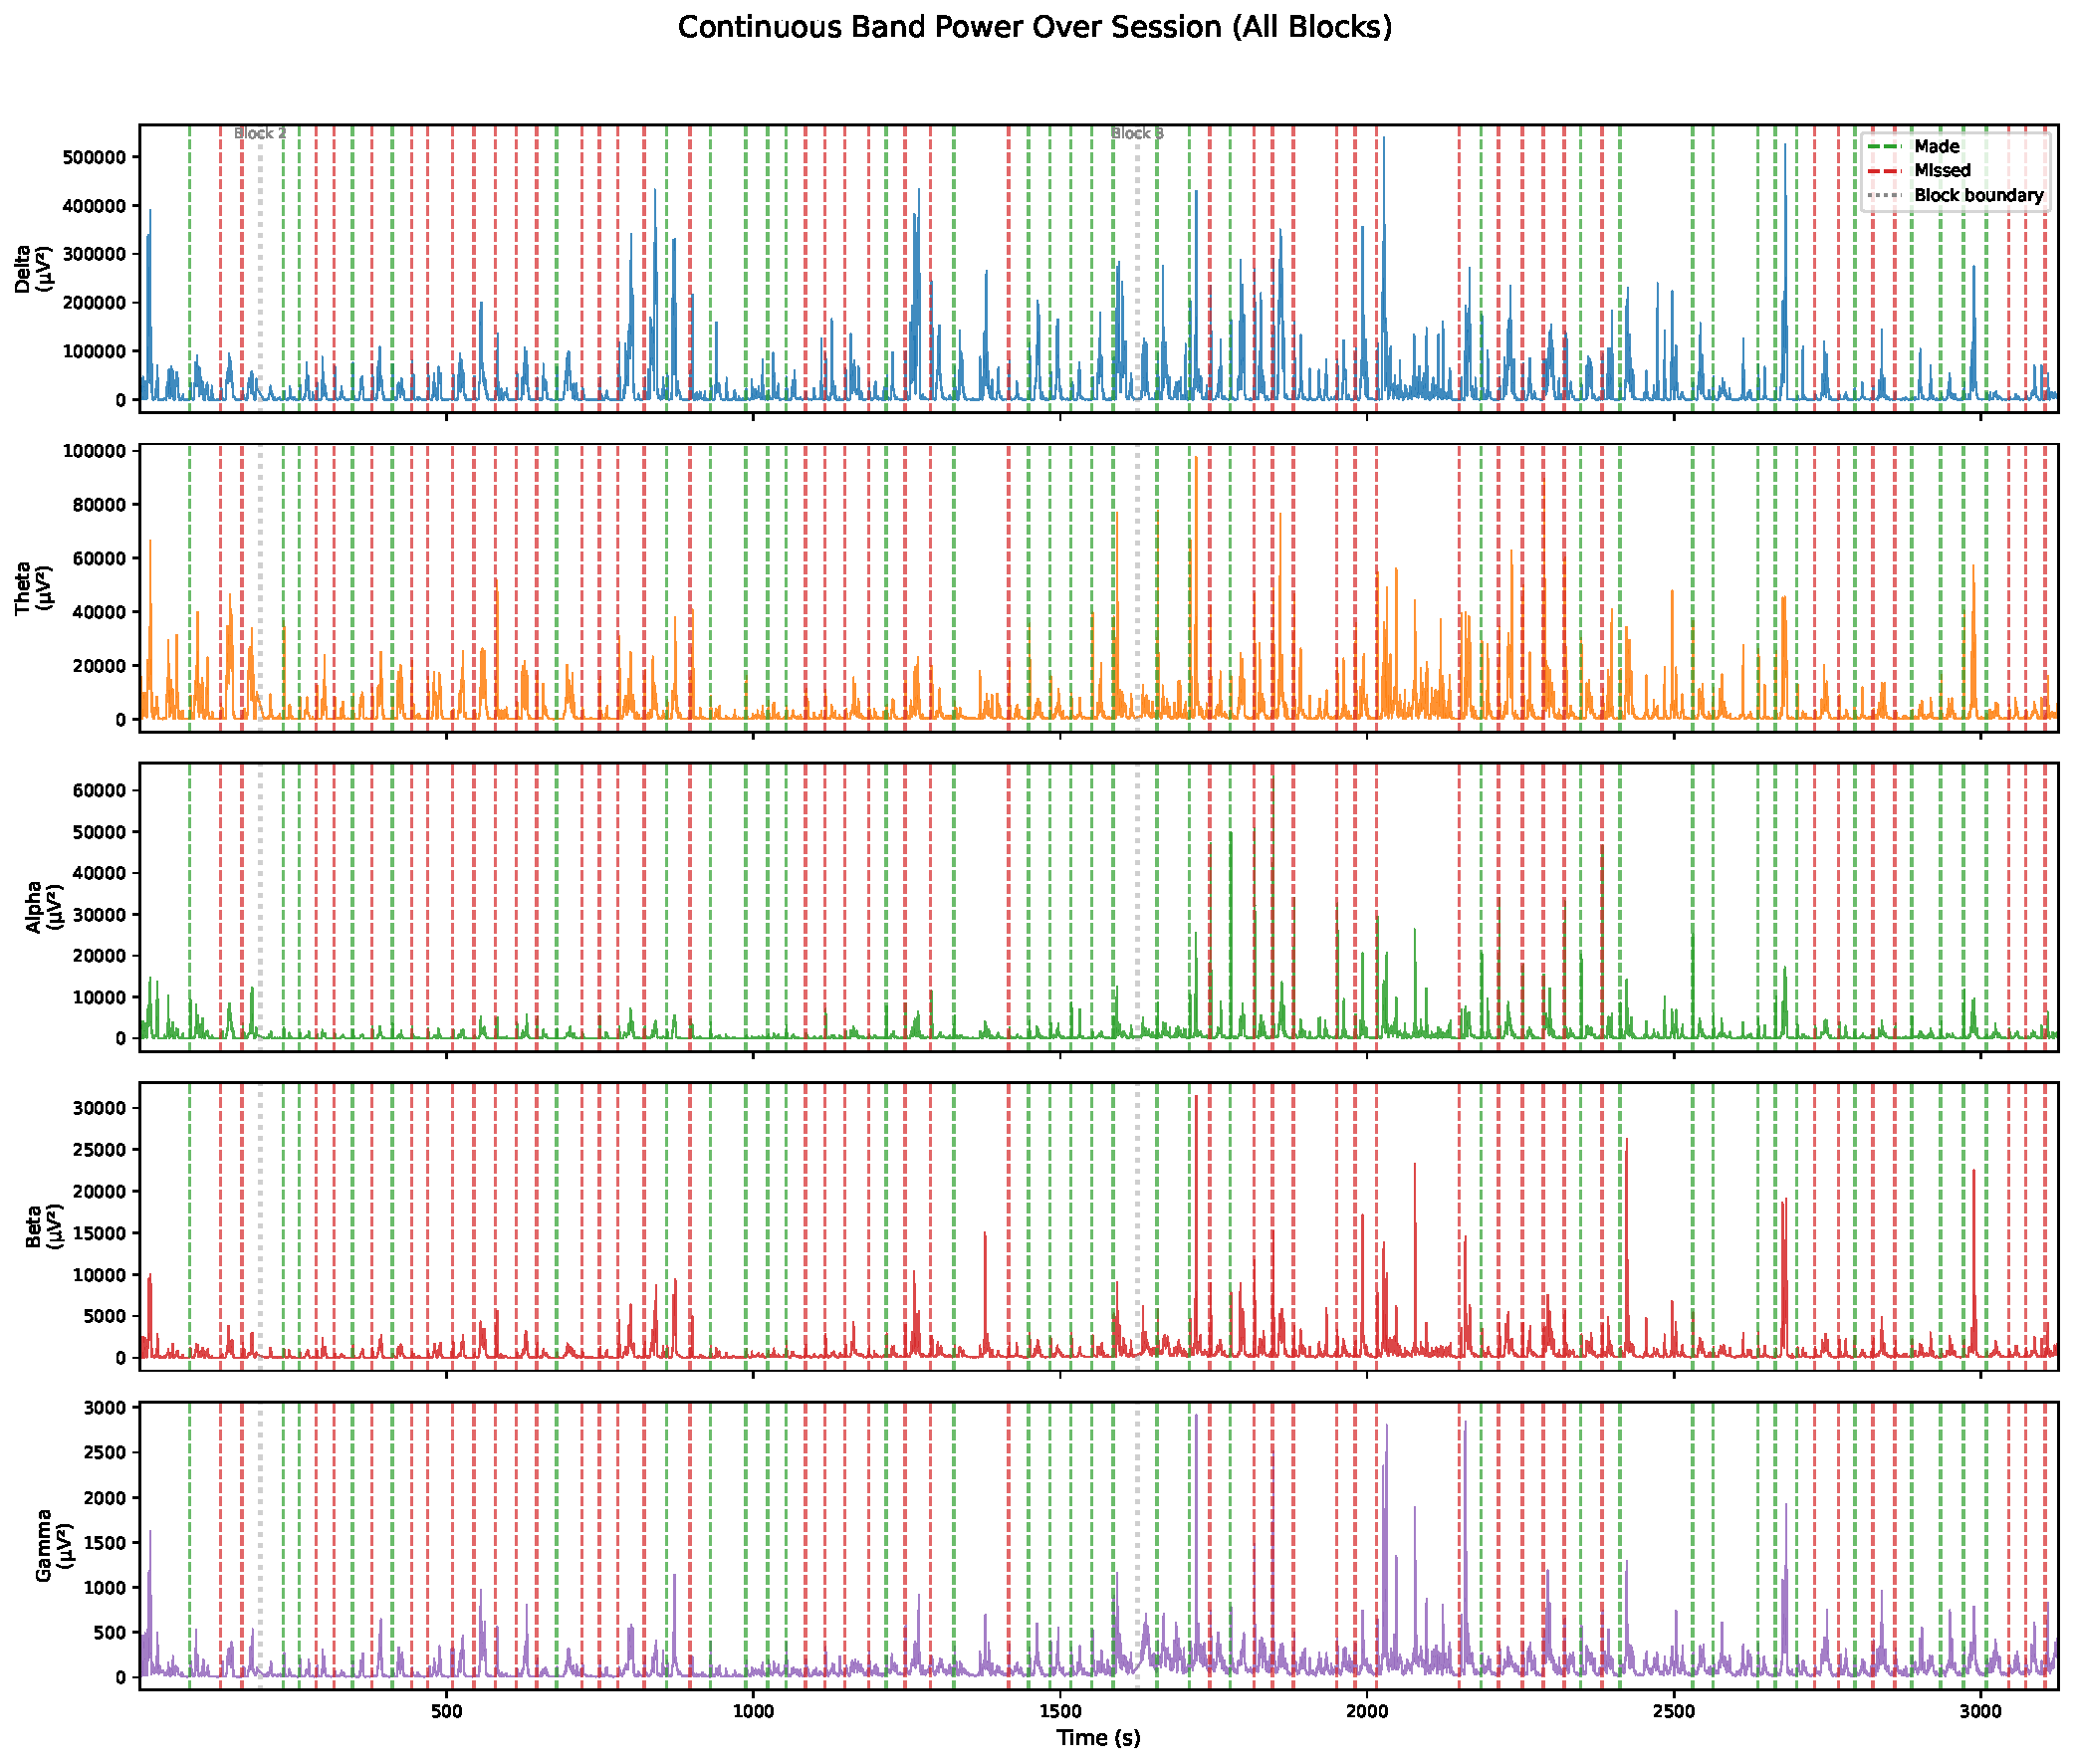
\includegraphics[width=\textwidth]{figures/fig_continuous_power.pdf}
  \caption{Continuous band power (delta through gamma) over all blocks. Band
  power was computed offline from the average of four electrode channels.
  Dashed vertical lines indicate shot execution (green = made, red = missed).}
  \label{fig:continuous}
\end{figure}

\subsection{Signal Filtering}
Figure~\ref{fig:filtering} demonstrates the effect of low-pass, high-pass, and
bandpass Butterworth filtering applied to the raw delta-band signal from the
first 60 seconds of recording.

\begin{figure}[H]
  \centering
  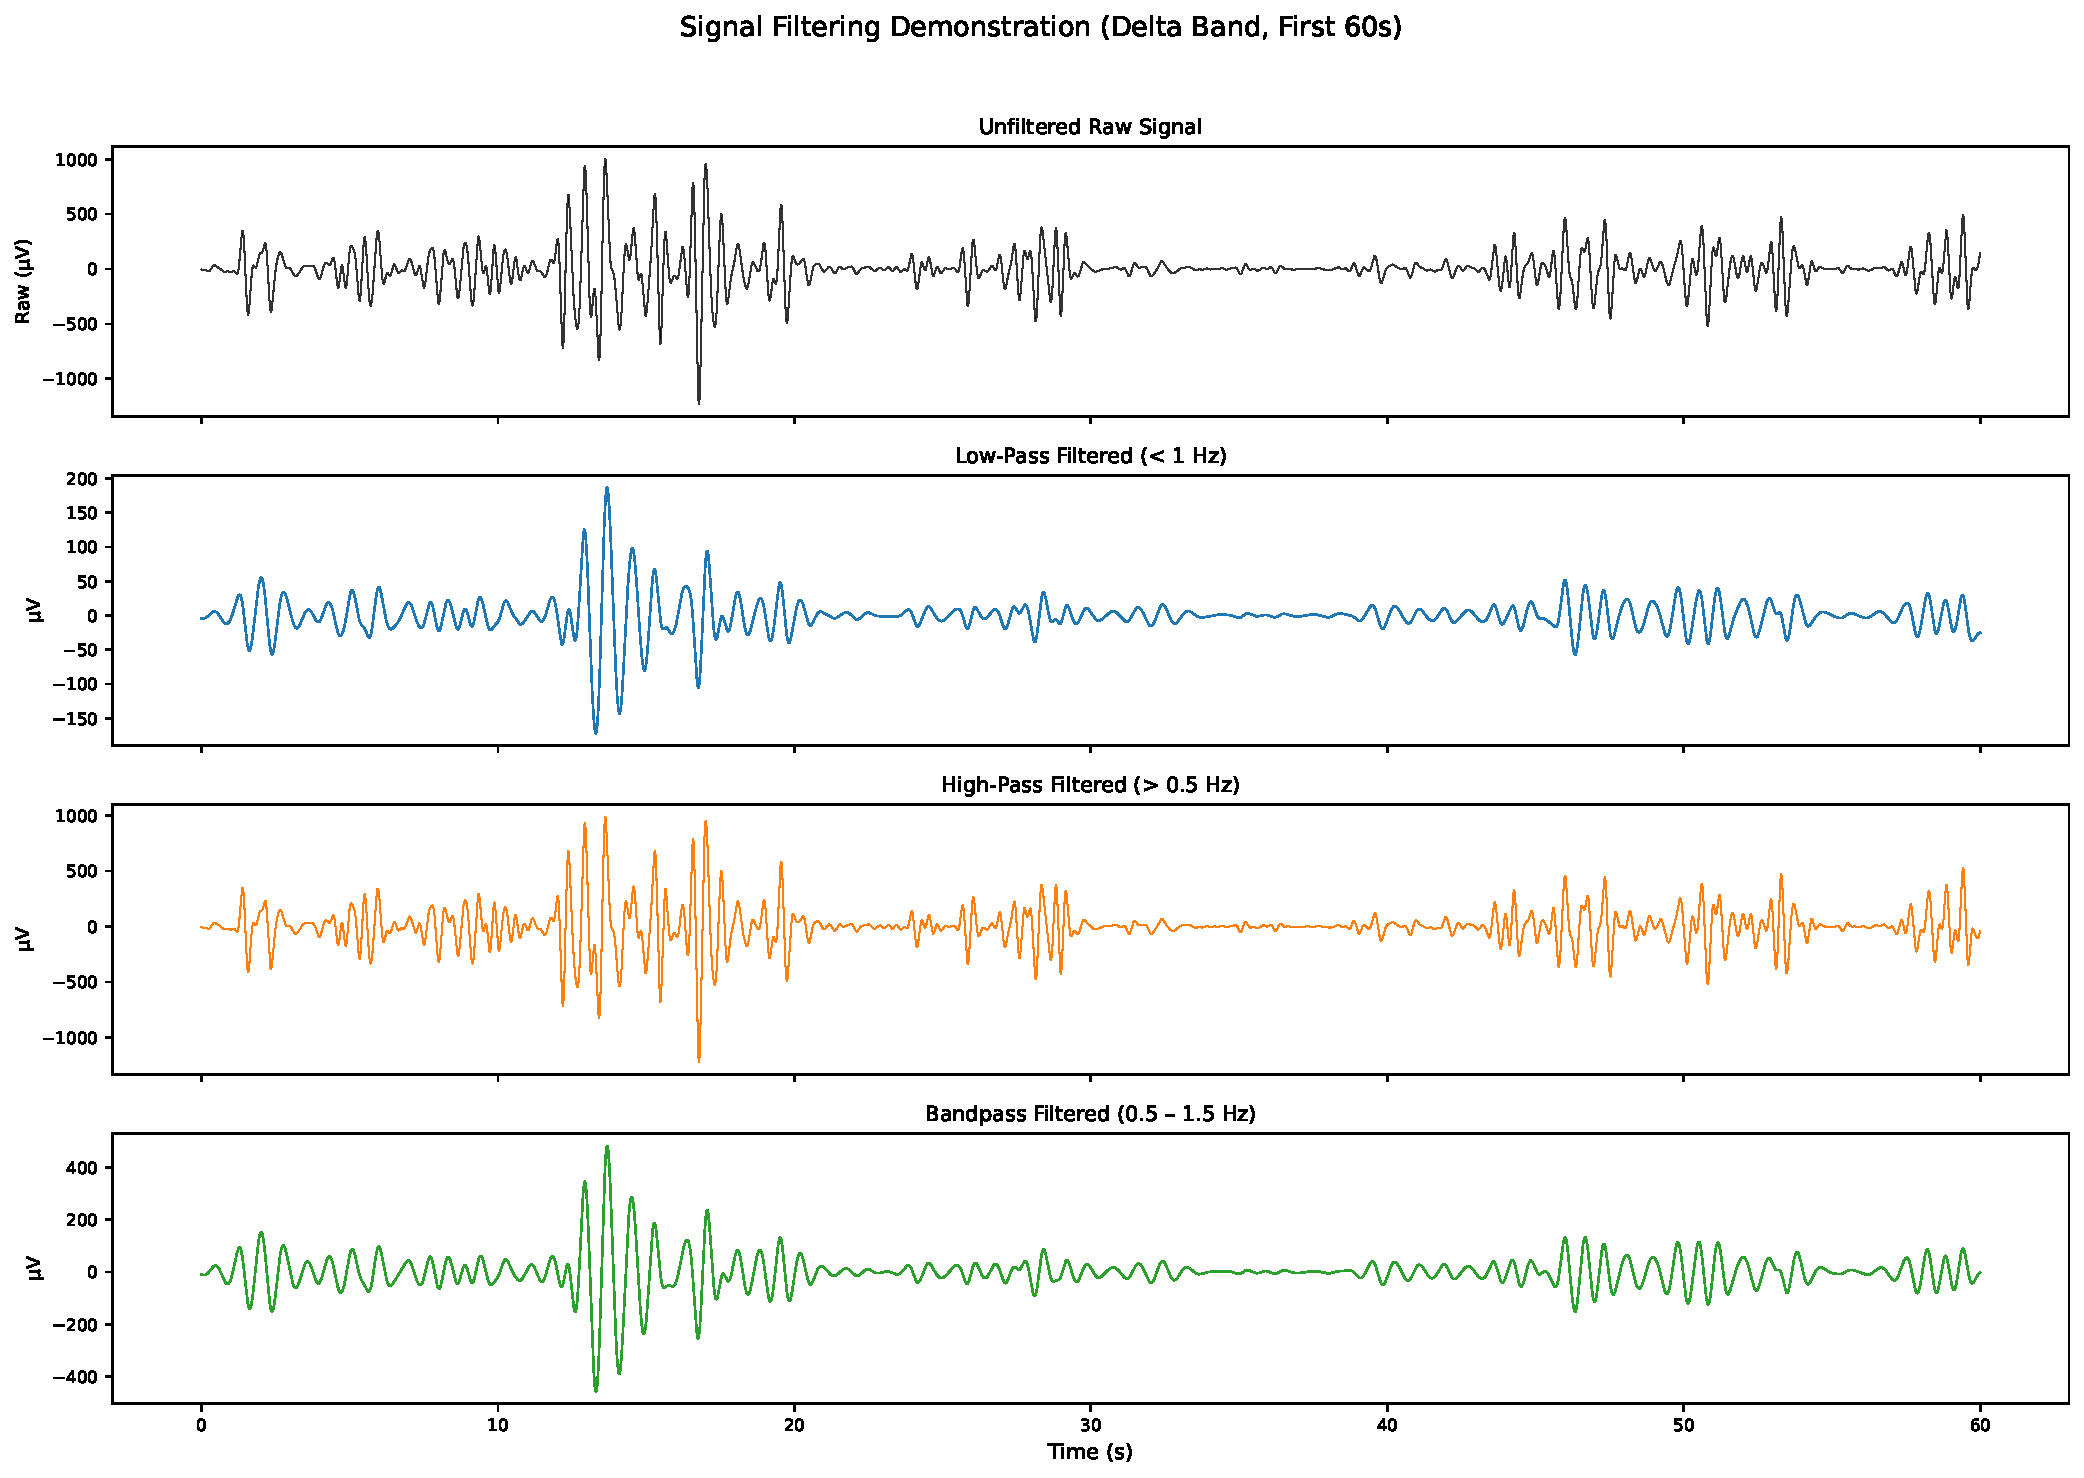
\includegraphics[width=\textwidth]{figures/fig_raw_filtering.pdf}
  \caption{Filtering demonstration on the raw delta signal: (a) unfiltered,
  (b) low-pass $<$1\,Hz, (c) high-pass $>$0.5\,Hz,
  (d) bandpass 0.5--1.5\,Hz.}
  \label{fig:filtering}
\end{figure}

\subsection{Shot-Locked Averages}
Figure~\ref{fig:shotlocked} shows mean band power ($\pm$ SEM) locked to the
onset of the execution phase, averaged across all 78 shots from all
blocks.

\begin{figure}[H]
  \centering
  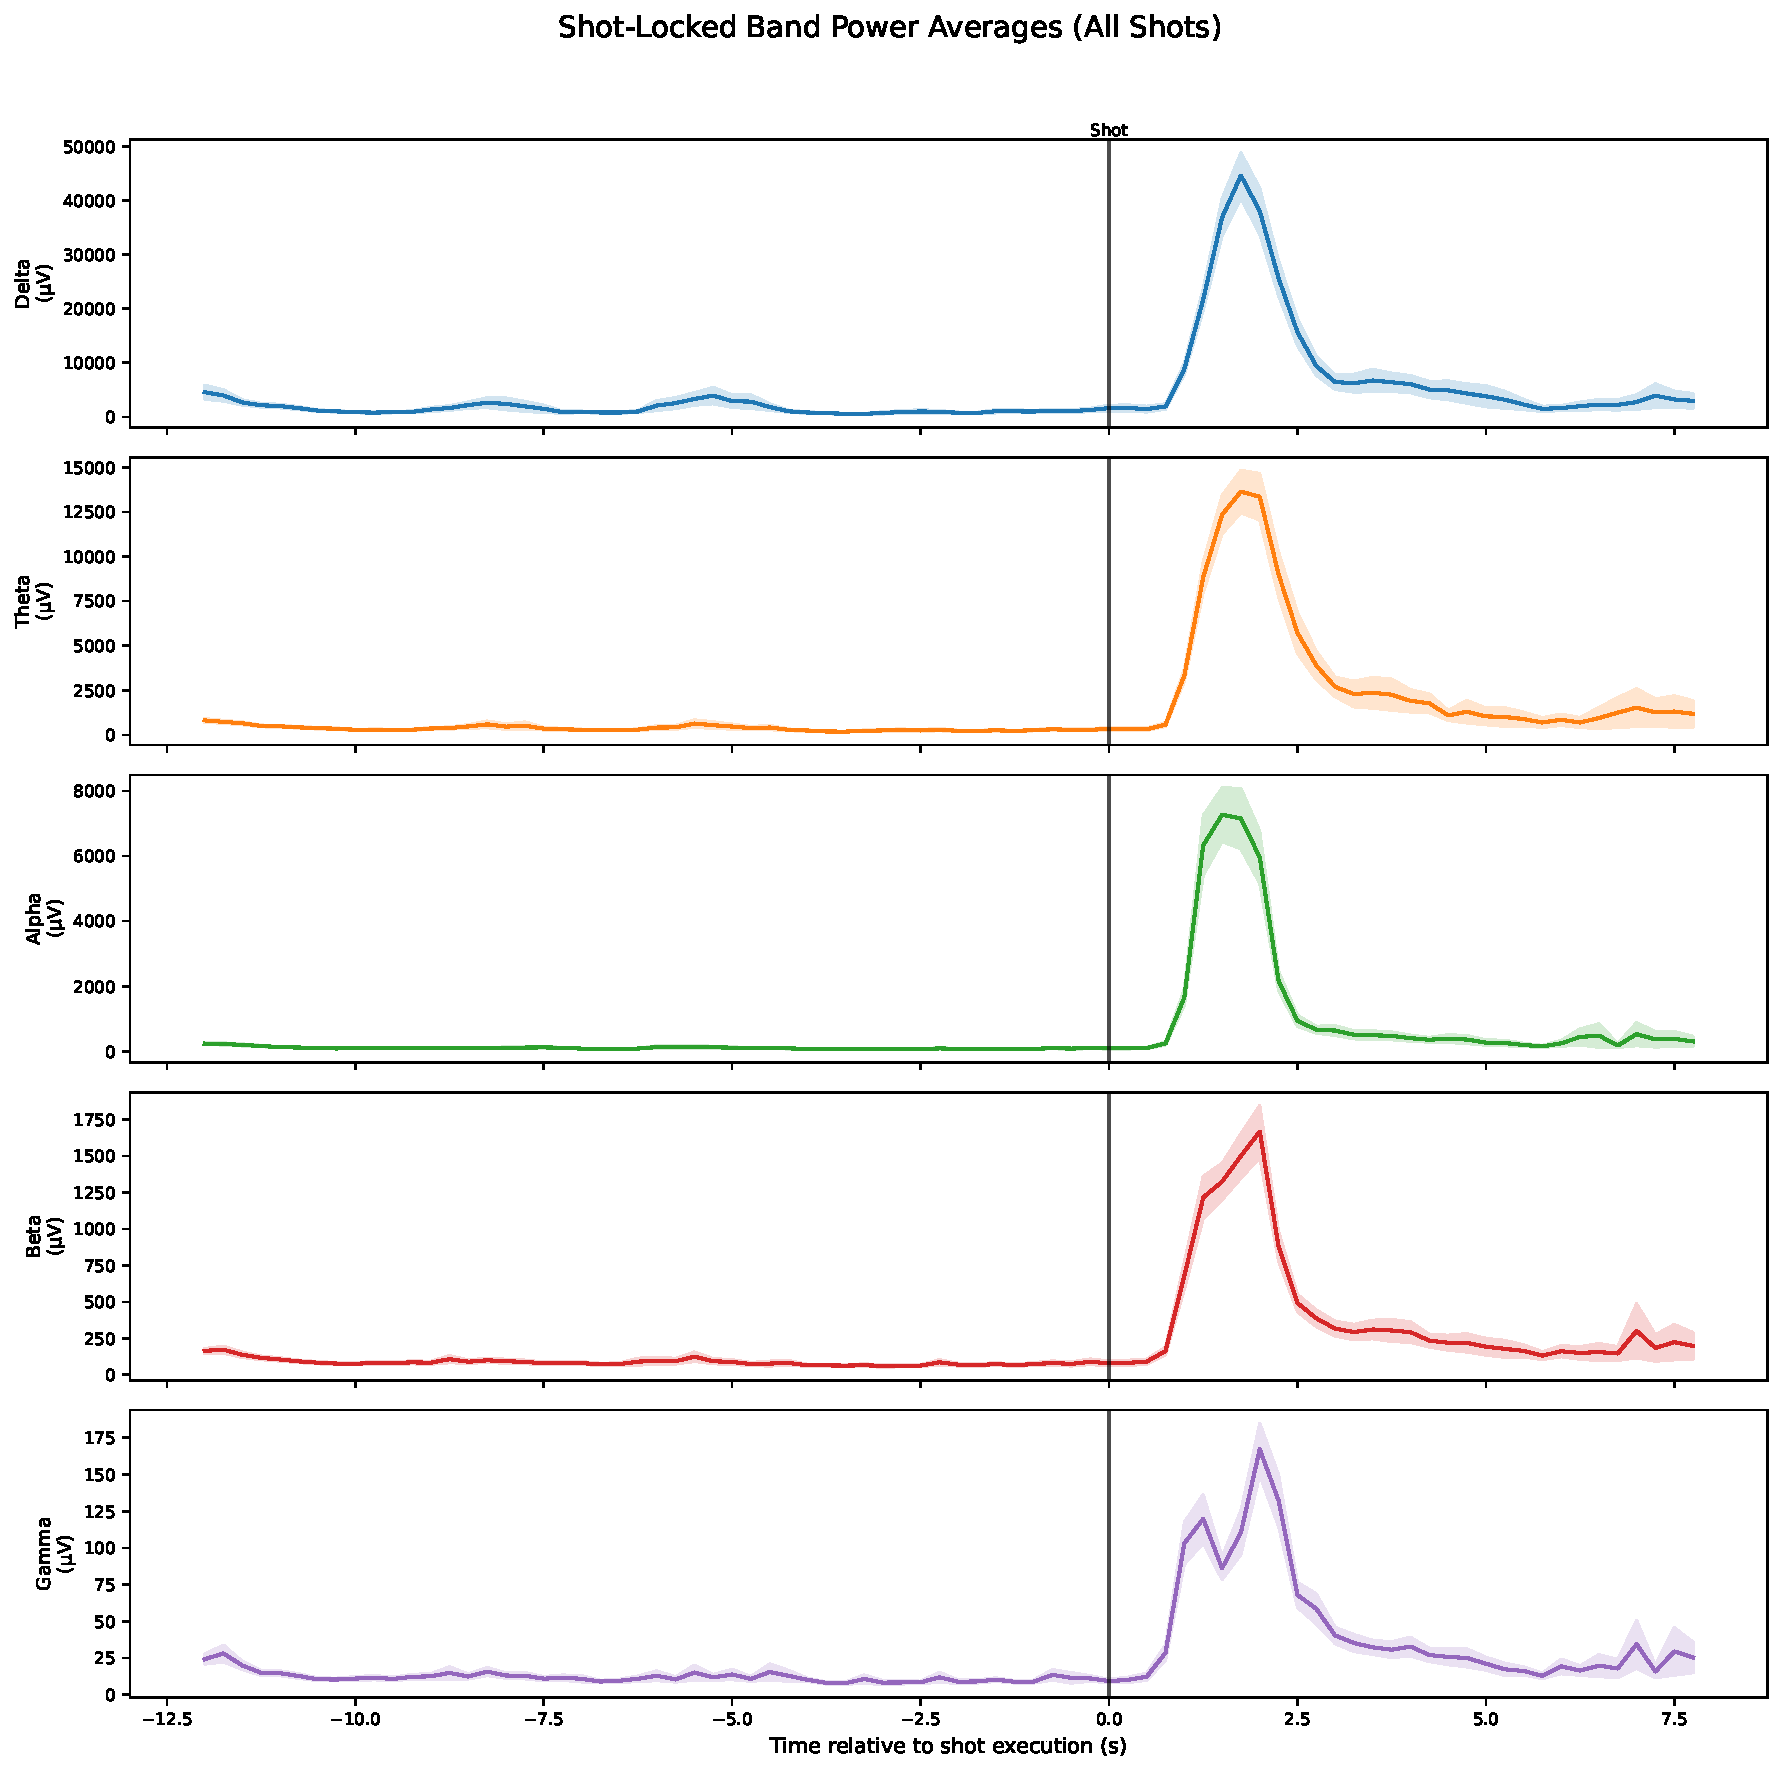
\includegraphics[width=\textwidth]{figures/fig_shot_locked_average.pdf}
  \caption{Shot-locked band power averages (all shots). Time 0 = execution
  onset. Shaded regions represent $\pm$1 SEM.}
  \label{fig:shotlocked}
\end{figure}

\subsection{Made vs.\ Missed Comparison}
Figure~\ref{fig:madevsmissed} compares shot-locked averages for made and missed
shots. delta power was 50.9\% higher for made shots ($M = 1717.7$) compared to missed ($M = 1138.0$). theta power was 39.6\% higher for made shots ($M = 390.4$) compared to missed ($M = 279.5$). alpha power was 16.7\% higher for made shots ($M = 105.9$) compared to missed ($M = 90.8$). beta power was 9.7\% higher for made shots ($M = 84.7$) compared to missed ($M = 77.2$). gamma power was 6.9\% higher for made shots ($M = 11.6$) compared to missed ($M = 10.9$). No frequency band reached trend-level significance ($p < .10$) in the pre-shot comparison, consistent with the limited sample size.

\begin{figure}[H]
  \centering
  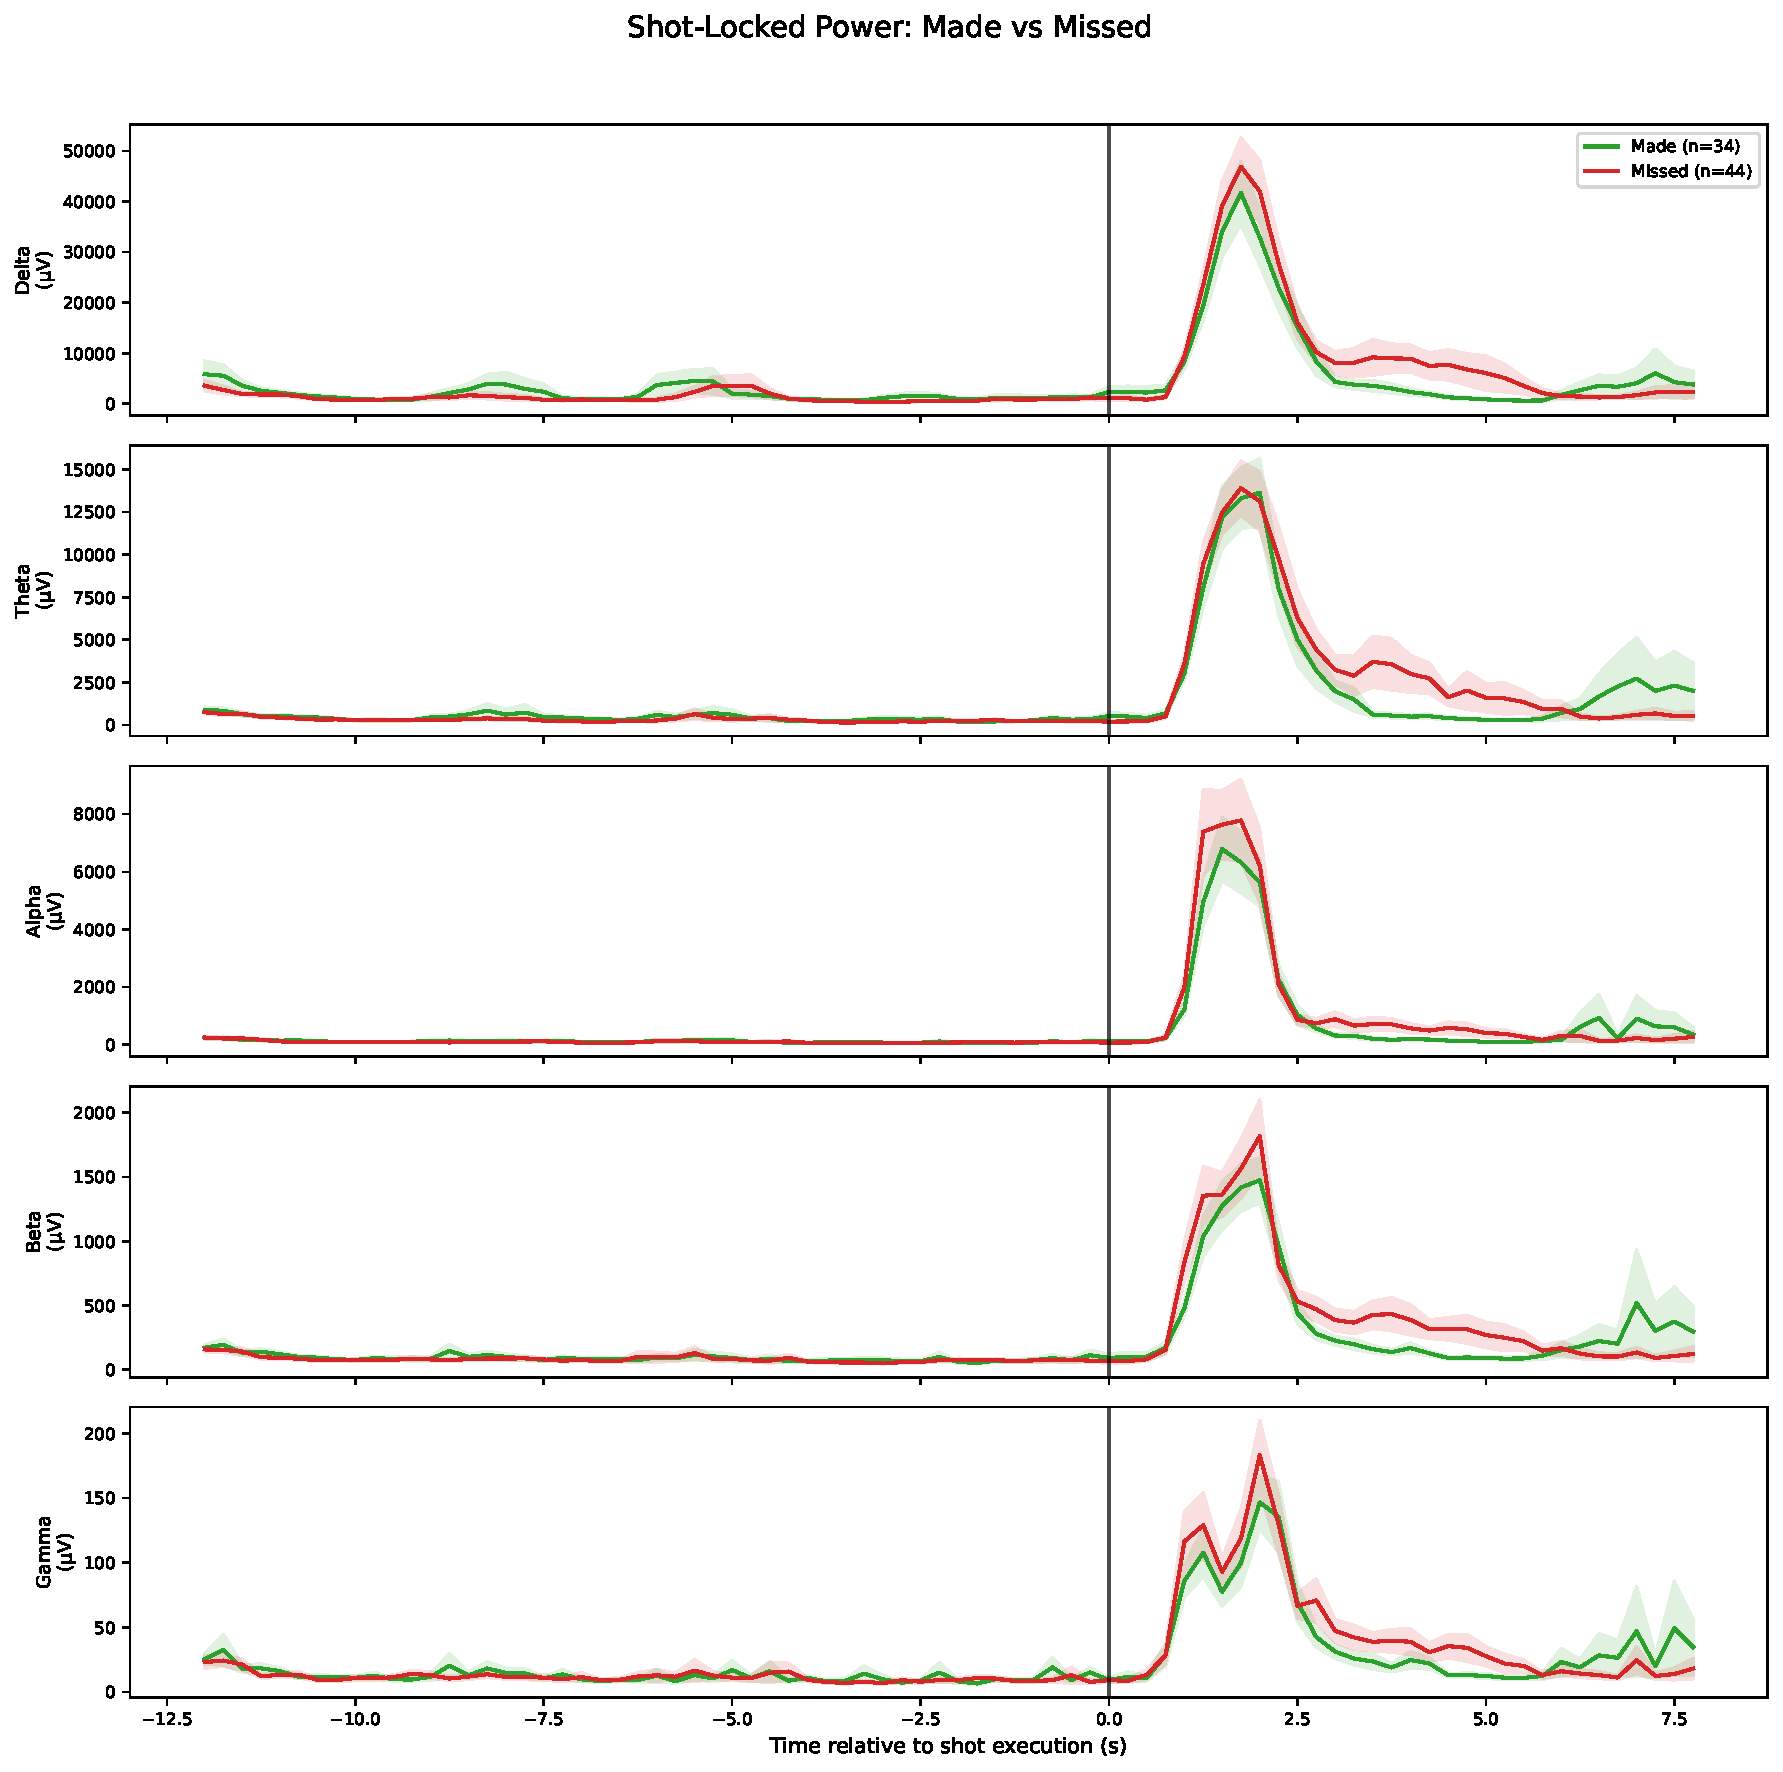
\includegraphics[width=\textwidth]{figures/fig_success_vs_failure.pdf}
  \caption{Shot-locked power comparison: made (green) vs.\ missed (red).
  Shaded regions are $\pm$1 SEM.}
  \label{fig:madevsmissed}
\end{figure}

\subsection{Phase-Wise Analysis}
Figure~\ref{fig:phasebars} displays mean power during the pre-shot, execution,
and post-shot phases, broken down by outcome and frequency band.
For made shots, delta power increased by 828.5\% from pre-shot to execution. For made shots, theta power increased by 1358.7\% from pre-shot to execution. For made shots, alpha power increased by 2205.9\% from pre-shot to execution. For made shots, beta power increased by 667.9\% from pre-shot to execution. For made shots, gamma power increased by 491.2\% from pre-shot to execution.

\begin{figure}[H]
  \centering
  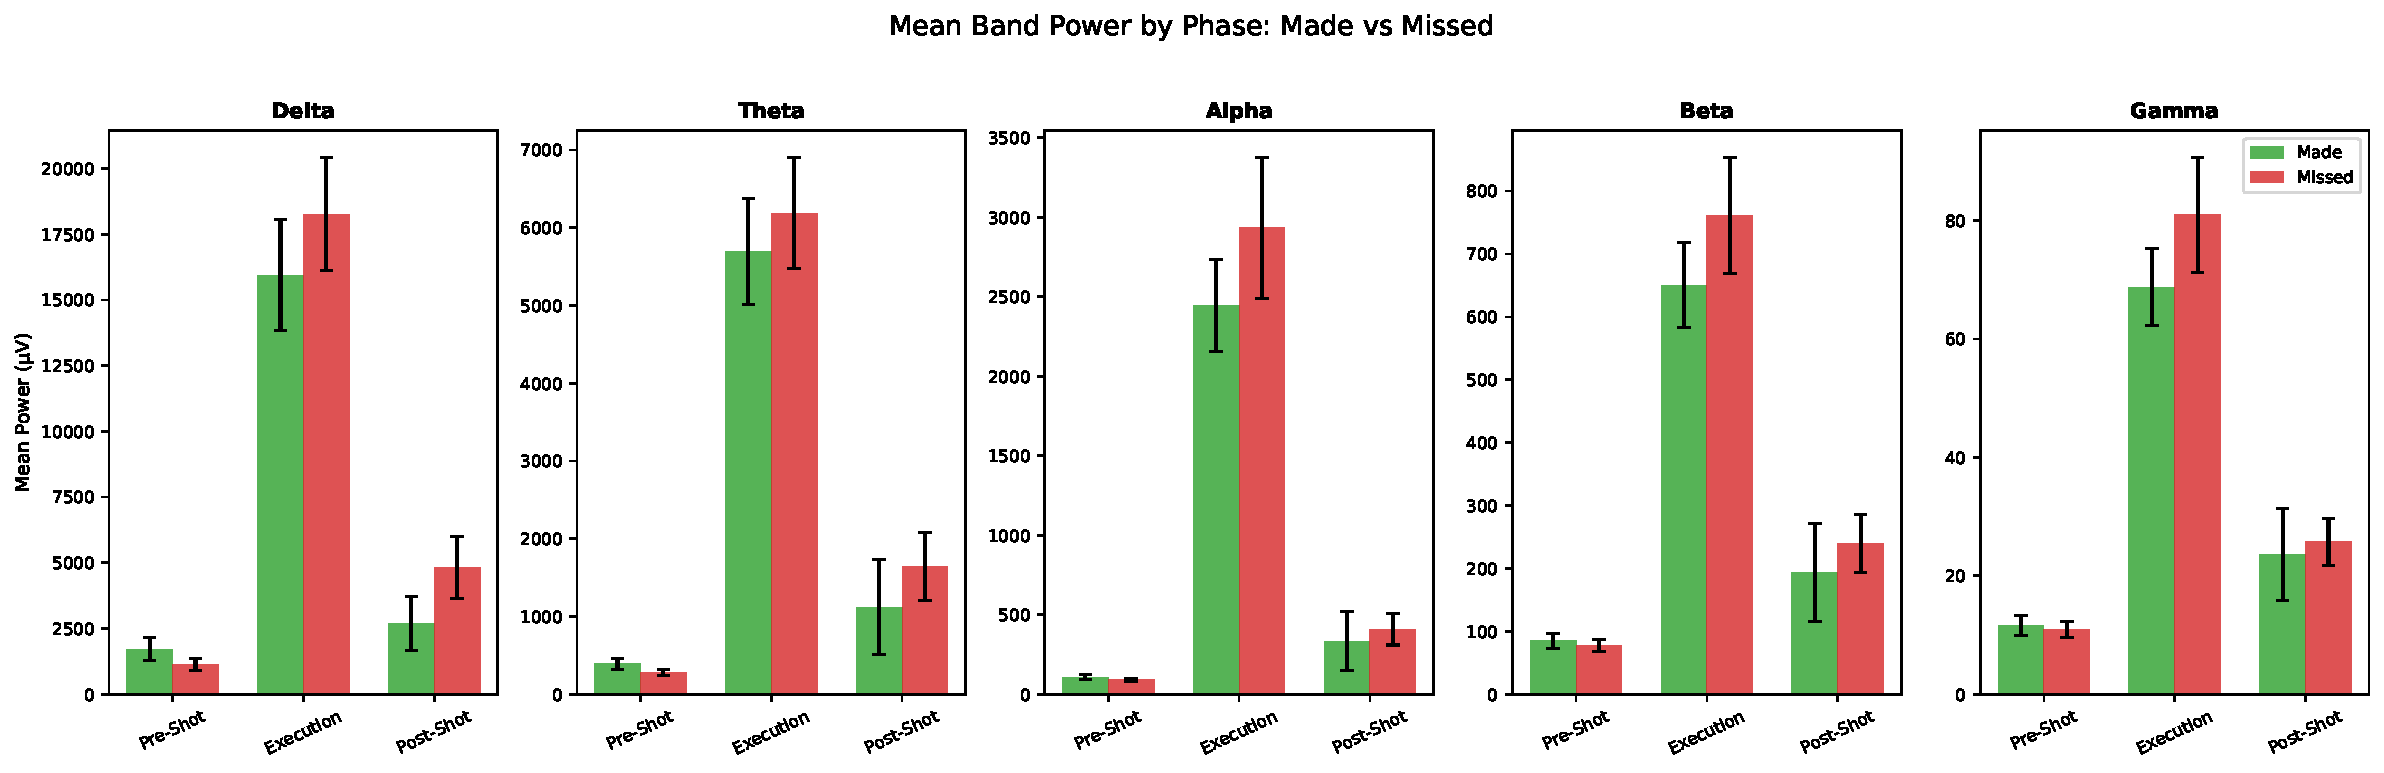
\includegraphics[width=\textwidth]{figures/fig_phase_bars.pdf}
  \caption{Mean band power by phase and outcome ($\pm$ SEM).}
  \label{fig:phasebars}
\end{figure}

\subsection{Statistical Comparisons}
Table~\ref{tab:stats} summarizes pre-shot band power for made and missed shots,
along with inferential test results.

\begin{table}[H]
\centering
\caption{Pre-shot band power: descriptive and inferential statistics.}
\label{tab:stats}
\small
\begin{tabular}{lcccccc}
\toprule
Band & Made $M$ (SD) & Missed $M$ (SD) & $t$ & $p$ & $U$ & $d$ \\
\midrule
Delta & 1717.7 (2600.6) & 1138.0 (1577.9) & 1.15 & 0.257 & 846 & 0.28 \\
Theta & 390.4 (426.2) & 279.5 (243.1) & 1.36 & 0.182 & 818 & 0.33 \\
Alpha & 105.9 (89.3) & 90.8 (69.5) & 0.82 & 0.416 & 789 & 0.19 \\
Beta & 84.7 (72.3) & 77.2 (63.2) & 0.48 & 0.633 & 766 & 0.11 \\
Gamma & 11.6 (10.0) & 10.9 (9.0) & 0.34 & 0.733 & 748 & 0.08 \\
\bottomrule
\end{tabular}
\end{table}

\subsection{Theta/Alpha Ratio}
The pre-shot theta/alpha ratio has been proposed as an index of focused attention in sport performance.. Mean pre-shot $\theta/\alpha$ ratio was 3.53 (SD = 1.25) for made shots and 3.24 (SD = 0.98) for missed shots. Made shots showed a higher $\theta/\alpha$ ratio, differing by 0.29.

\begin{figure}[H]
  \centering
  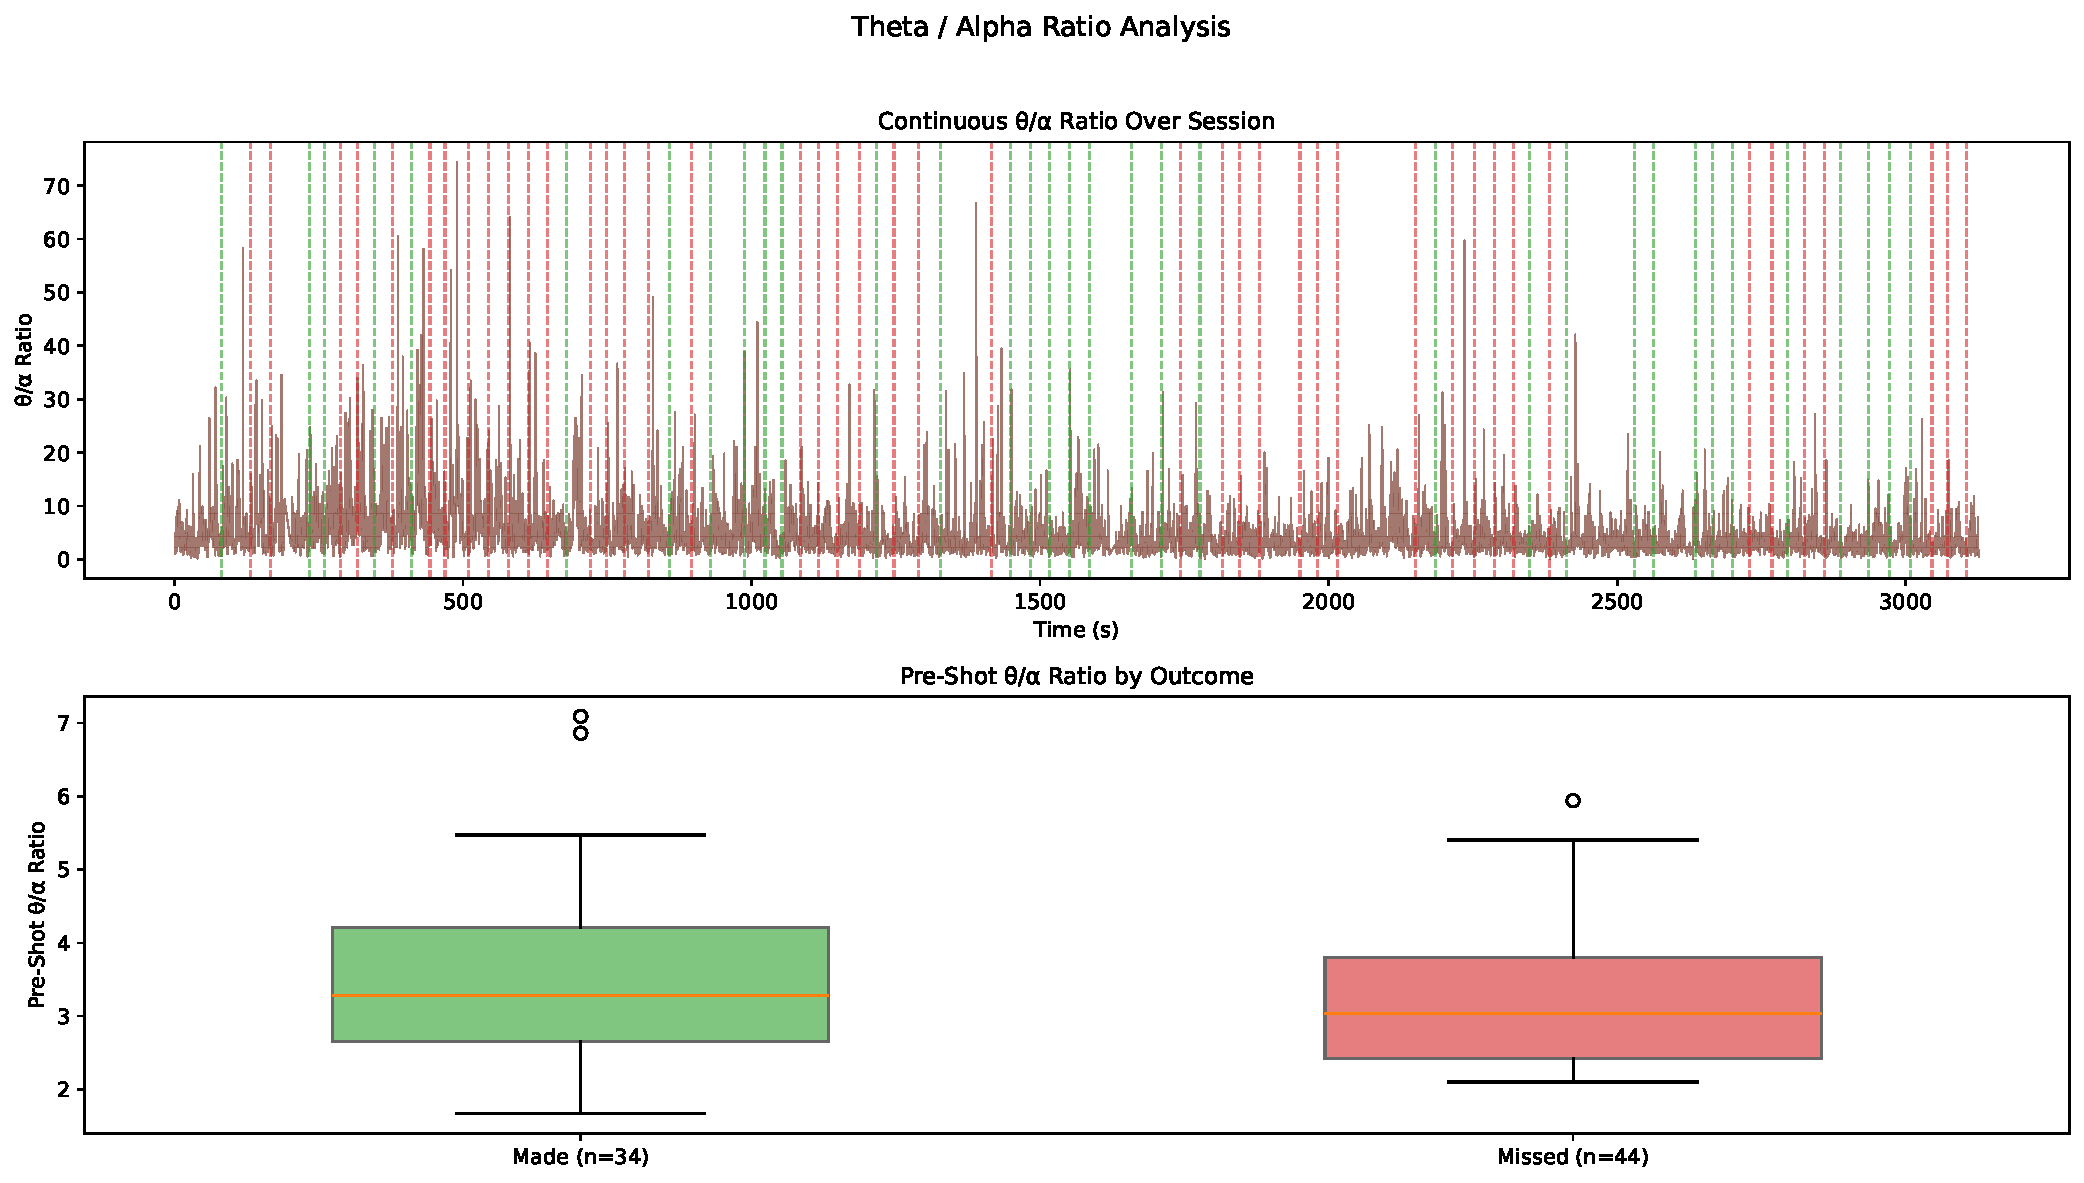
\includegraphics[width=\textwidth]{figures/fig_theta_alpha_ratio.pdf}
  \caption{(Top) Continuous $\theta/\alpha$ ratio over the session. (Bottom)
  Pre-shot $\theta/\alpha$ ratio by outcome.}
  \label{fig:thetaalpha}
\end{figure}

\subsection{Shot-by-Shot Progression}
Figure~\ref{fig:progression} tracks pre-shot band power across the 78
shots. Pre-shot alpha power showed a trend toward increase across the session ($r = 0.31$, $p = 0.006$), though the correlation was weak, possibly due to the limited number of trials.

\begin{figure}[H]
  \centering
  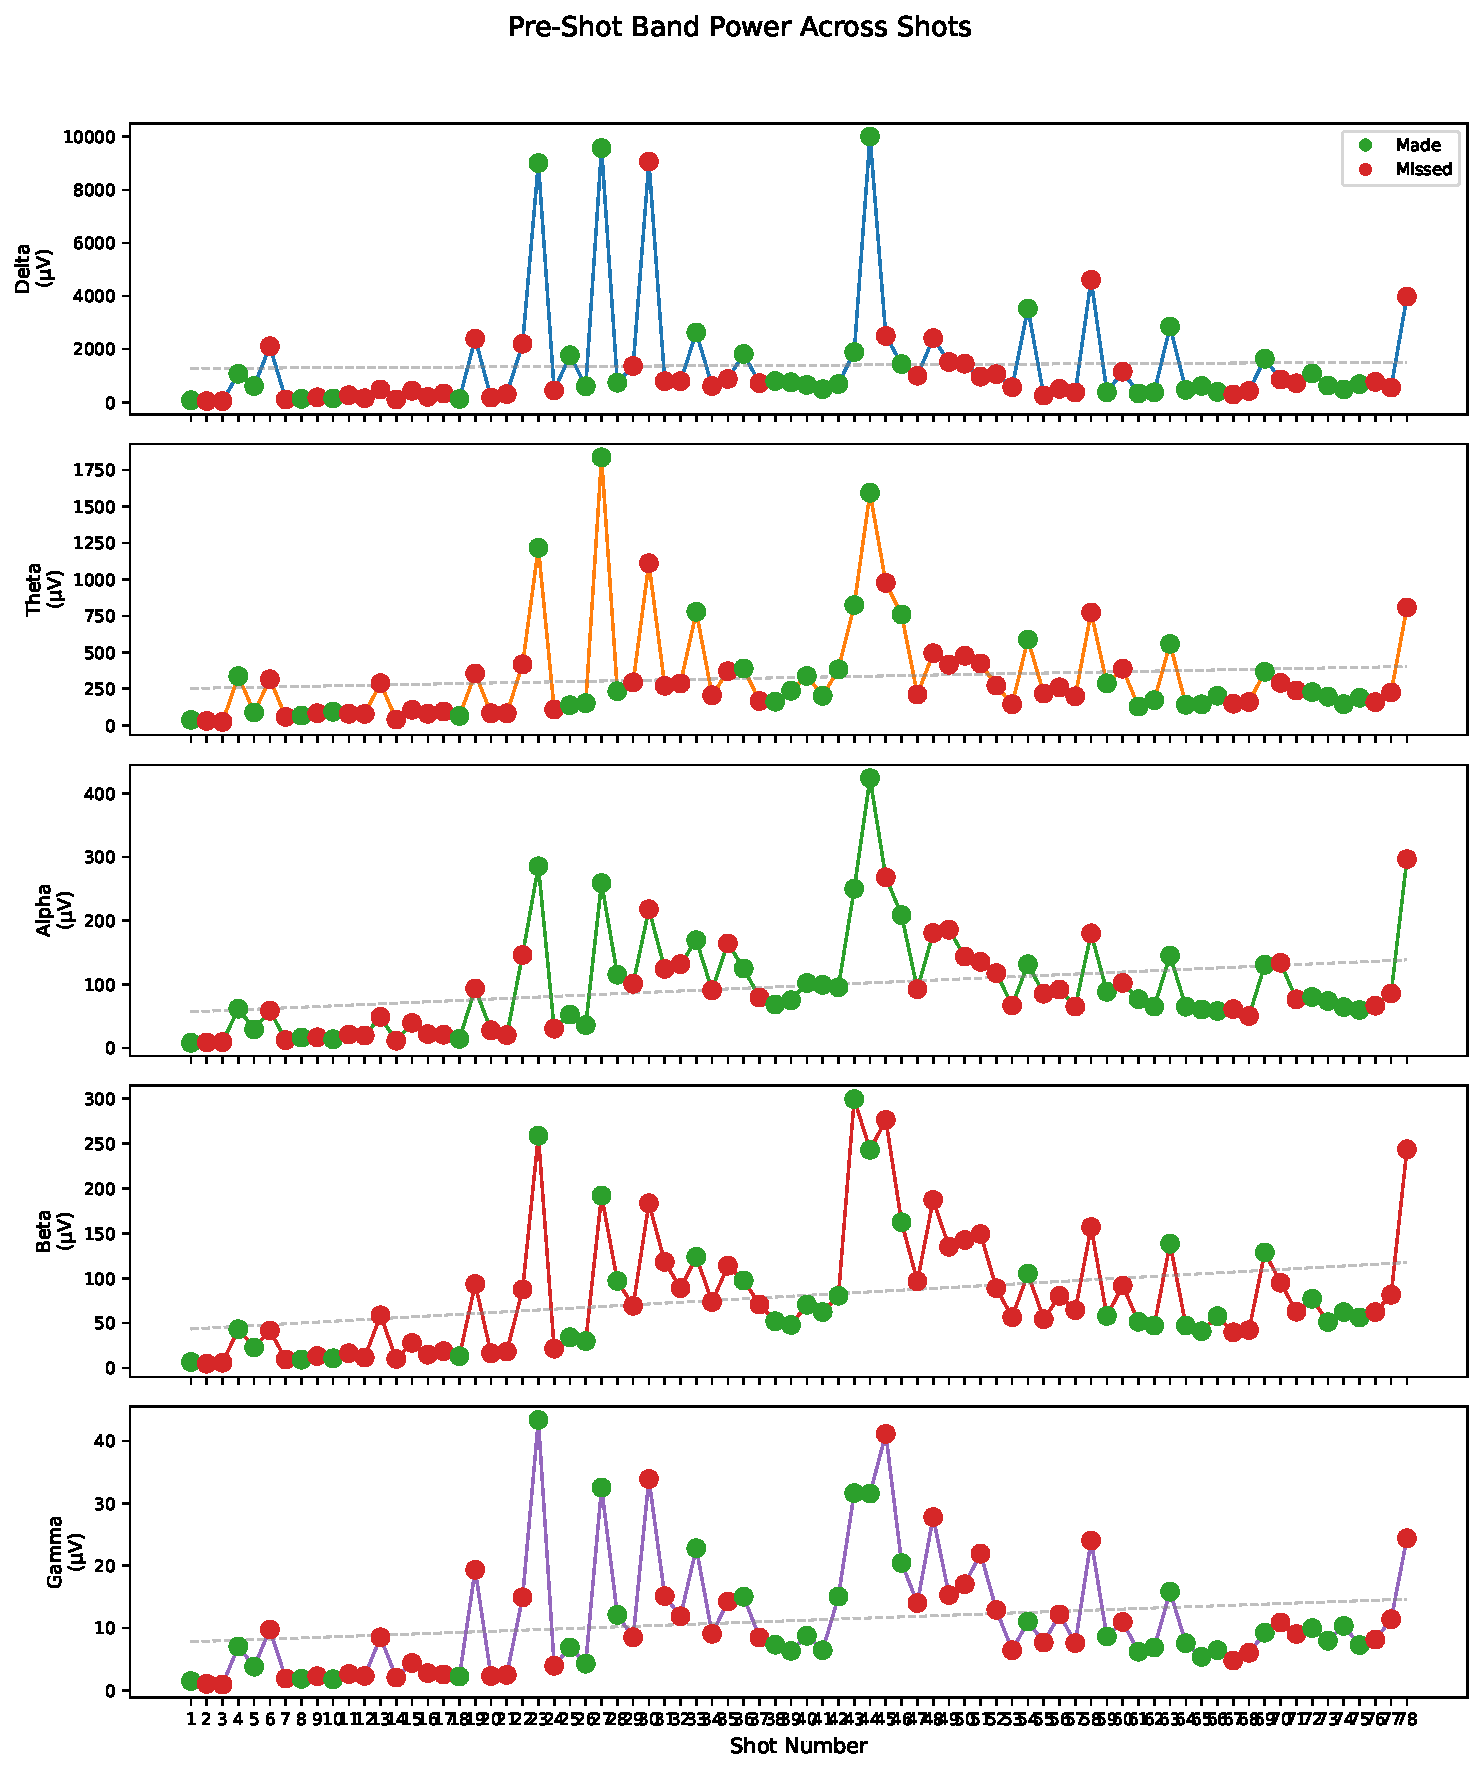
\includegraphics[width=\textwidth]{figures/fig_shot_progression.pdf}
  \caption{Pre-shot band power across shots. Dot colour indicates outcome
  (green = made, red = missed). Dashed line shows linear trend.}
  \label{fig:progression}
\end{figure}

% ────────────────────────────────────────────────────────────────────────────
\section{Video and Pose Estimation Analysis}

Video was recorded for Blocks~1 and 3, but not for Block~2 (video did not
save). Due to EEG timing synchronization issues in Block~1, video-based
analyses were performed on Block~3's 36 shots only. Post-hoc
pose estimation was performed using MediaPipe Pose (heavy model) to extract 33
body landmarks per frame. Biomechanical features---elbow angle, wrist height,
knee angle, and body lean angle---were computed across the shot execution phase
for each trial and compared between made and missed shots.

\subsection{Shot Stop-Motion Montage}
Figure~\ref{fig:montage} presents a frame-by-frame stop-motion decomposition
of each shot during the execution phase, with pose skeleton overlays. Made
shots are shown in the upper rows (green borders) and missed shots in the
lower rows (red borders).

\begin{figure}[H]
  \centering
  
\includegraphics[width=\textwidth]{figures/fig_shot_montage.pdf}
  \caption{Stop-motion montage of shots during the execution phase. Pose
  skeleton overlays are drawn semi-transparently. Border colour indicates
  outcome (green = made, red = missed).}
  \label{fig:montage}
\end{figure}

\subsection{Ghost Shot Overlay}
Figure~\ref{fig:ghost} shows composite ``ghost'' images created by pixel-averaging
the release-point frames across made and missed shots separately (top row),
along with skeleton-only overlays showing individual shot pose variability
(bottom row).

\begin{figure}[H]
  \centering
  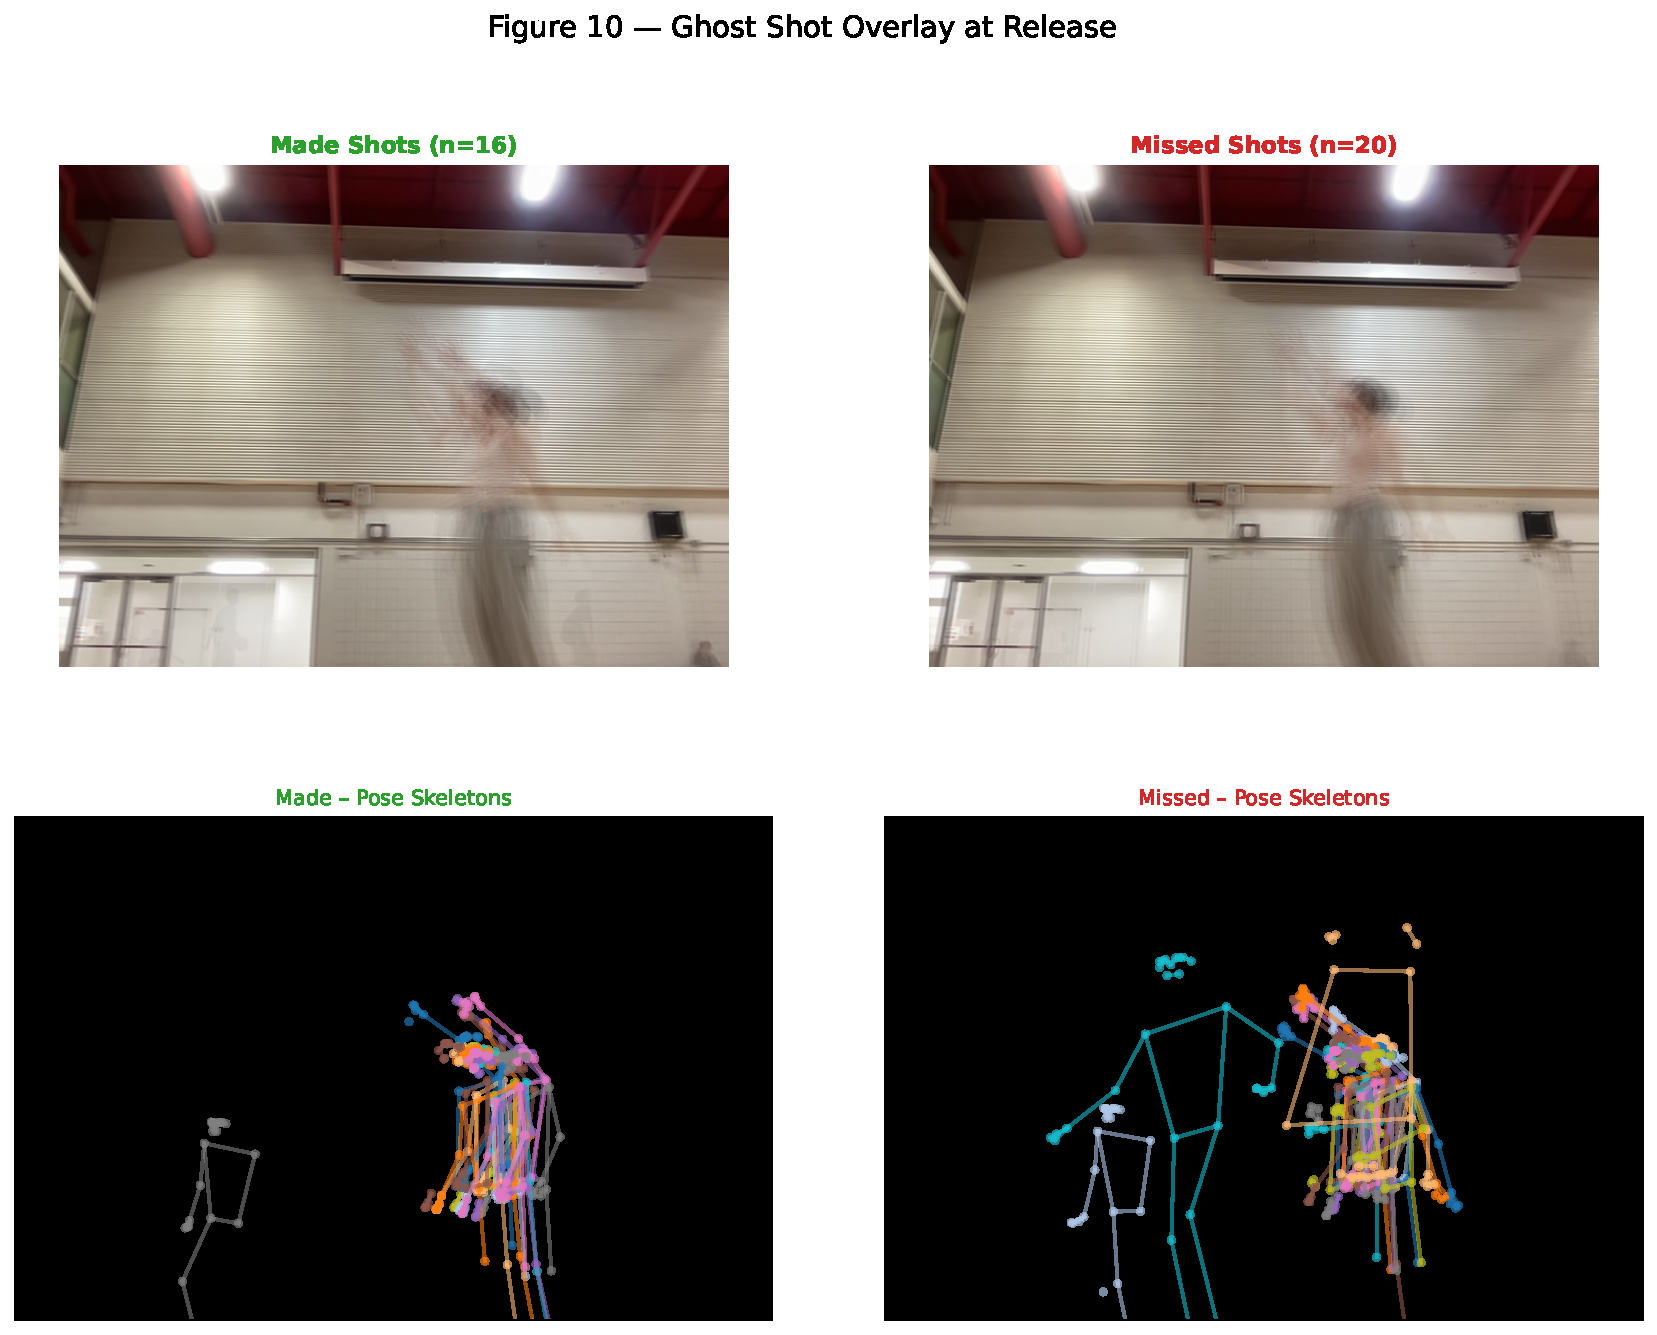
\includegraphics[width=\textwidth]{figures/fig_ghost_overlay.pdf}
  \caption{Ghost overlay composites at the estimated release point. Top:
  pixel-averaged frames for made (left) and missed (right) shots. Bottom:
  skeleton-only overlays with individual shots in distinct colours.}
  \label{fig:ghost}
\end{figure}

\subsection{Pose Kinematics Trajectories}
Figure~\ref{fig:kinematics} plots the time course of four biomechanical
features during the execution phase, comparing made (green) and missed (red)
shots. Peak elbow angle was lower for made shots (166.3) than missed (168.8). Peak wrist height was lower for made shots (0.4) than missed (0.5). Peak knee angle was lower for made shots (173.9) than missed (175.5). Peak body lean was lower for made shots (4.2) than missed (14.9).

\begin{figure}[H]
  \centering
  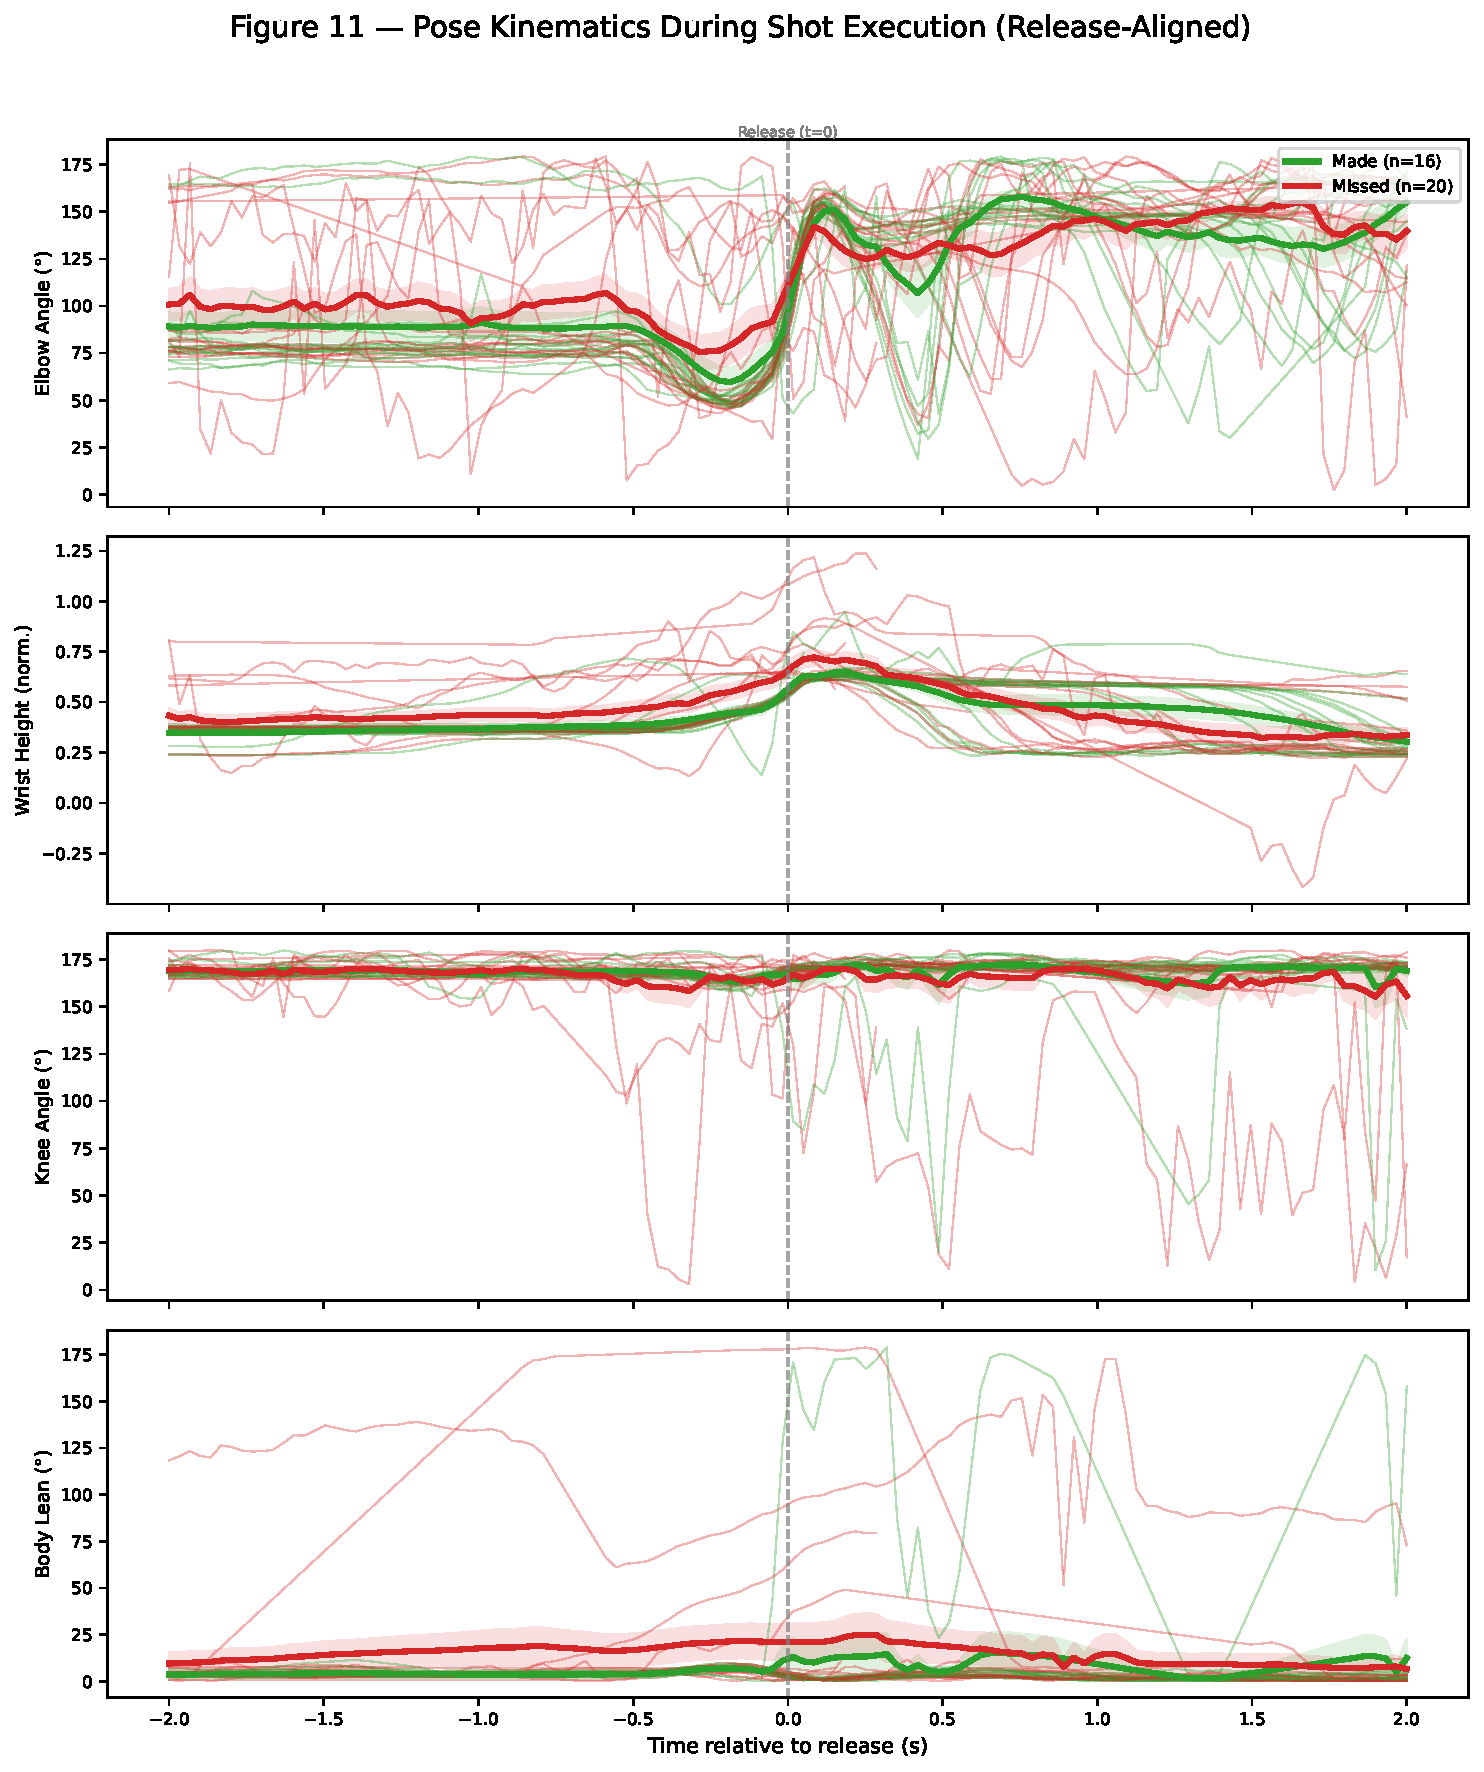
\includegraphics[width=\textwidth]{figures/fig_pose_kinematics.pdf}
  \caption{Biomechanical feature trajectories during shot execution (mean
  $\pm$ SEM). Thin lines show individual shots; thick lines show group means.
  Dashed vertical line: estimated release point.}
  \label{fig:kinematics}
\end{figure}

\subsection{Integrated Pose and EEG Analysis}
Figure~\ref{fig:poseeeg} presents a joint visualization of pose kinematics
(elbow angle, wrist height) and EEG dynamics (alpha power, $\theta/\alpha$
ratio) during the execution phase, time-aligned to recording onset.
Time-aligned visualization of pose and EEG data during execution reveals concurrent motor and neural dynamics. Cross-domain correlations between mean pose features and alpha power are annotated where available.

\begin{figure}[H]
  \centering
  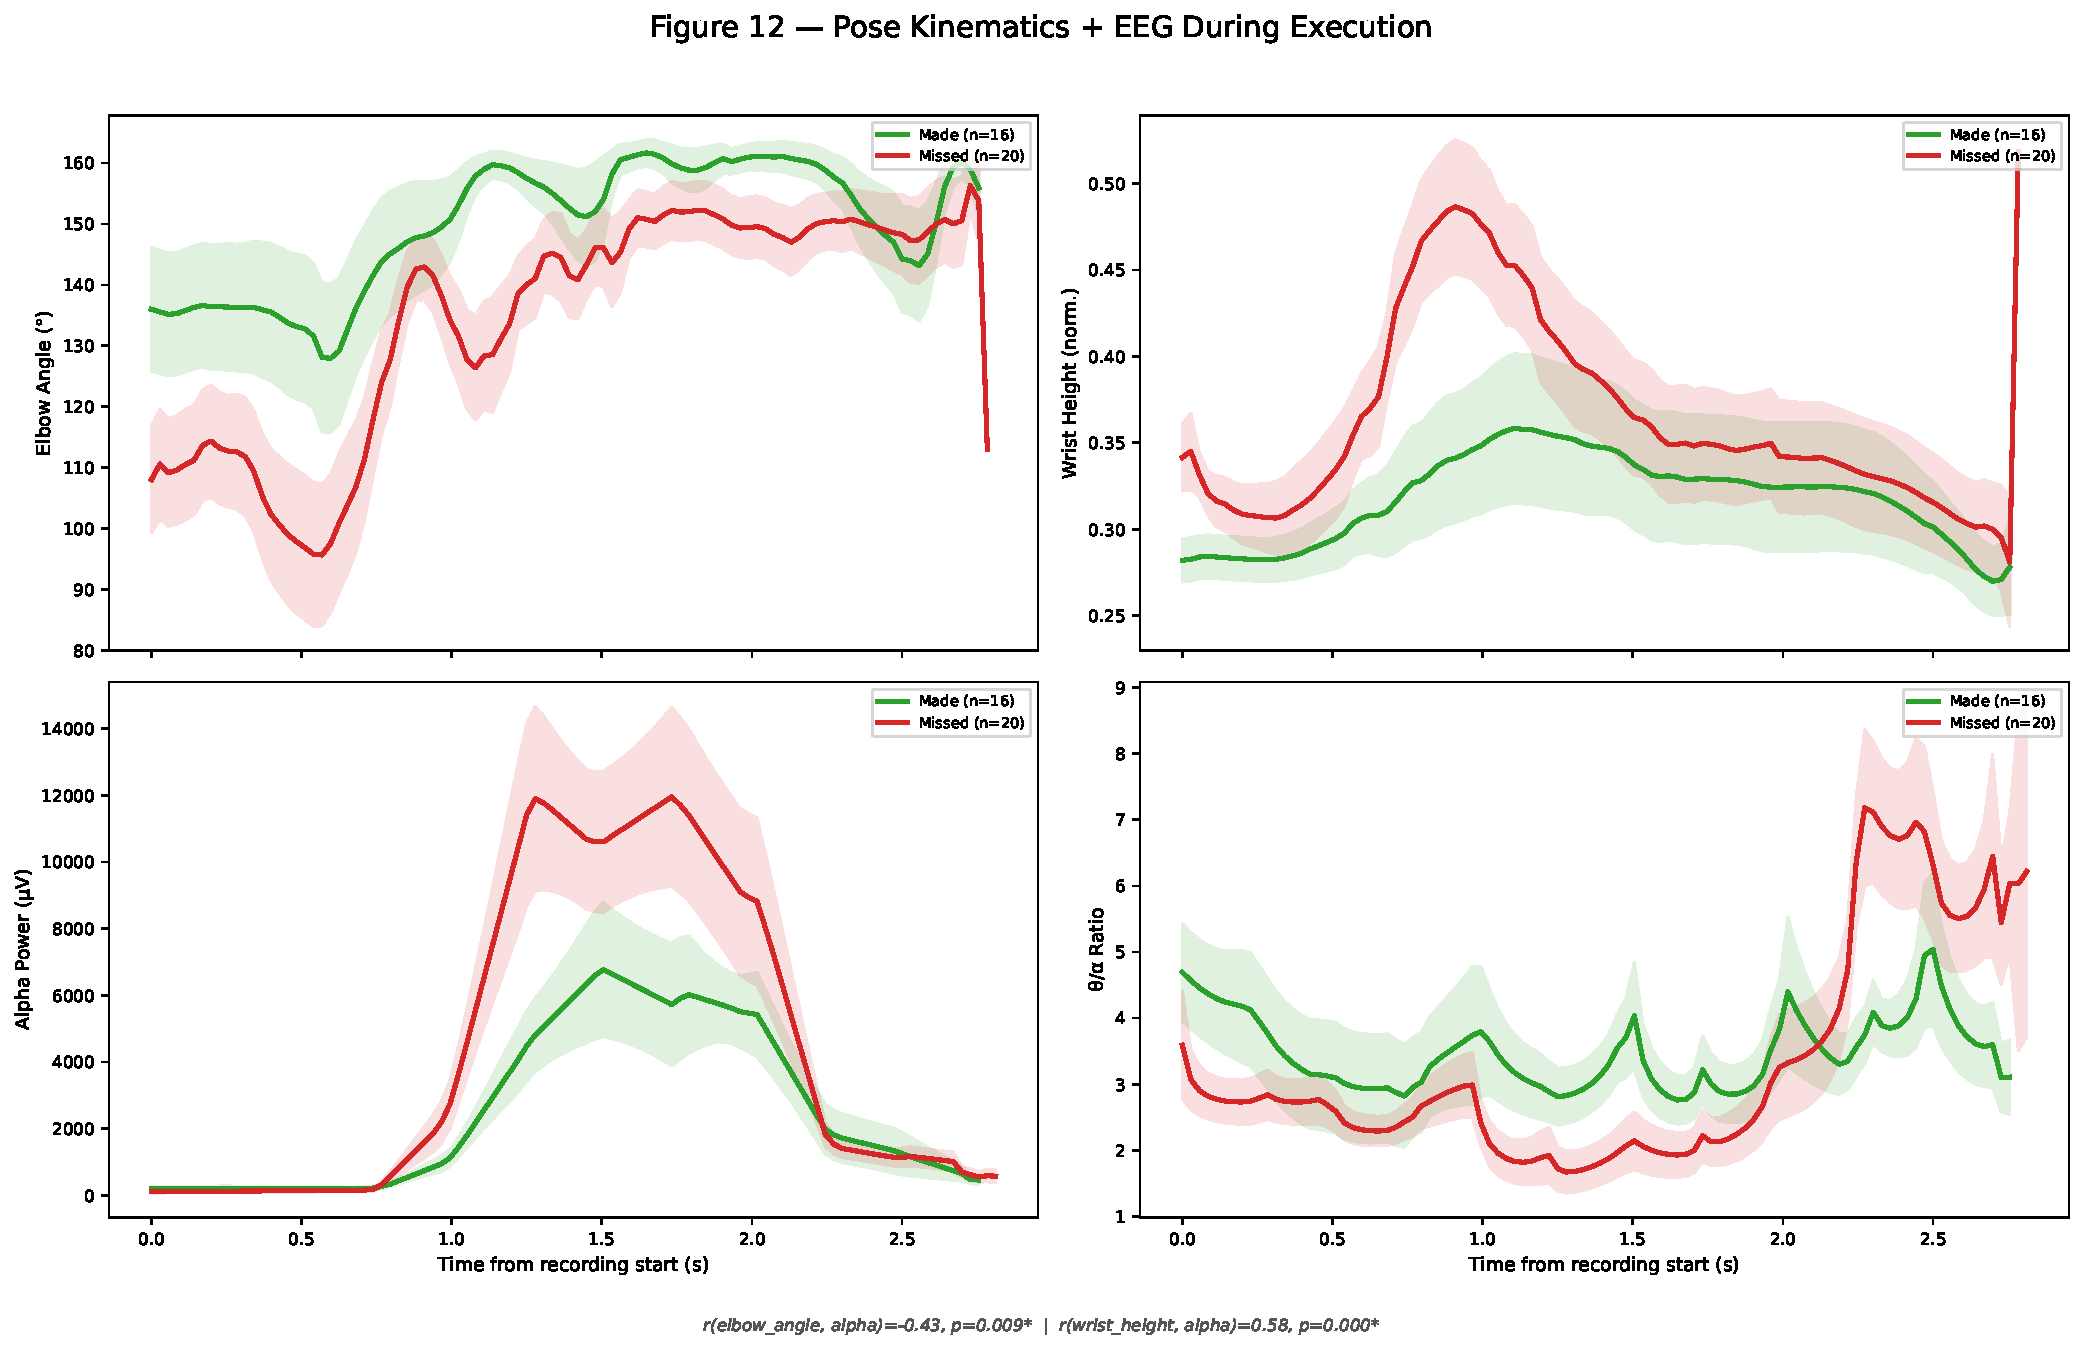
\includegraphics[width=\textwidth]{figures/fig_pose_eeg_combined.pdf}
  \caption{Combined pose kinematics and EEG dynamics during shot execution.
  Top row: elbow angle and wrist height. Bottom row: alpha band power and
  $\theta/\alpha$ ratio. All traces show made (green) vs.\ missed (red) mean
  $\pm$ SEM.}
  \label{fig:poseeeg}
\end{figure}

\subsection{Average Frame Composites}
Figure~\ref{fig:avgframes} shows pixel-averaged video frames at three time
points (start, midpoint, end) of the execution phase for made and missed shots,
with an absolute difference image highlighting regions of greatest divergence.

\begin{figure}[H]
  \centering
  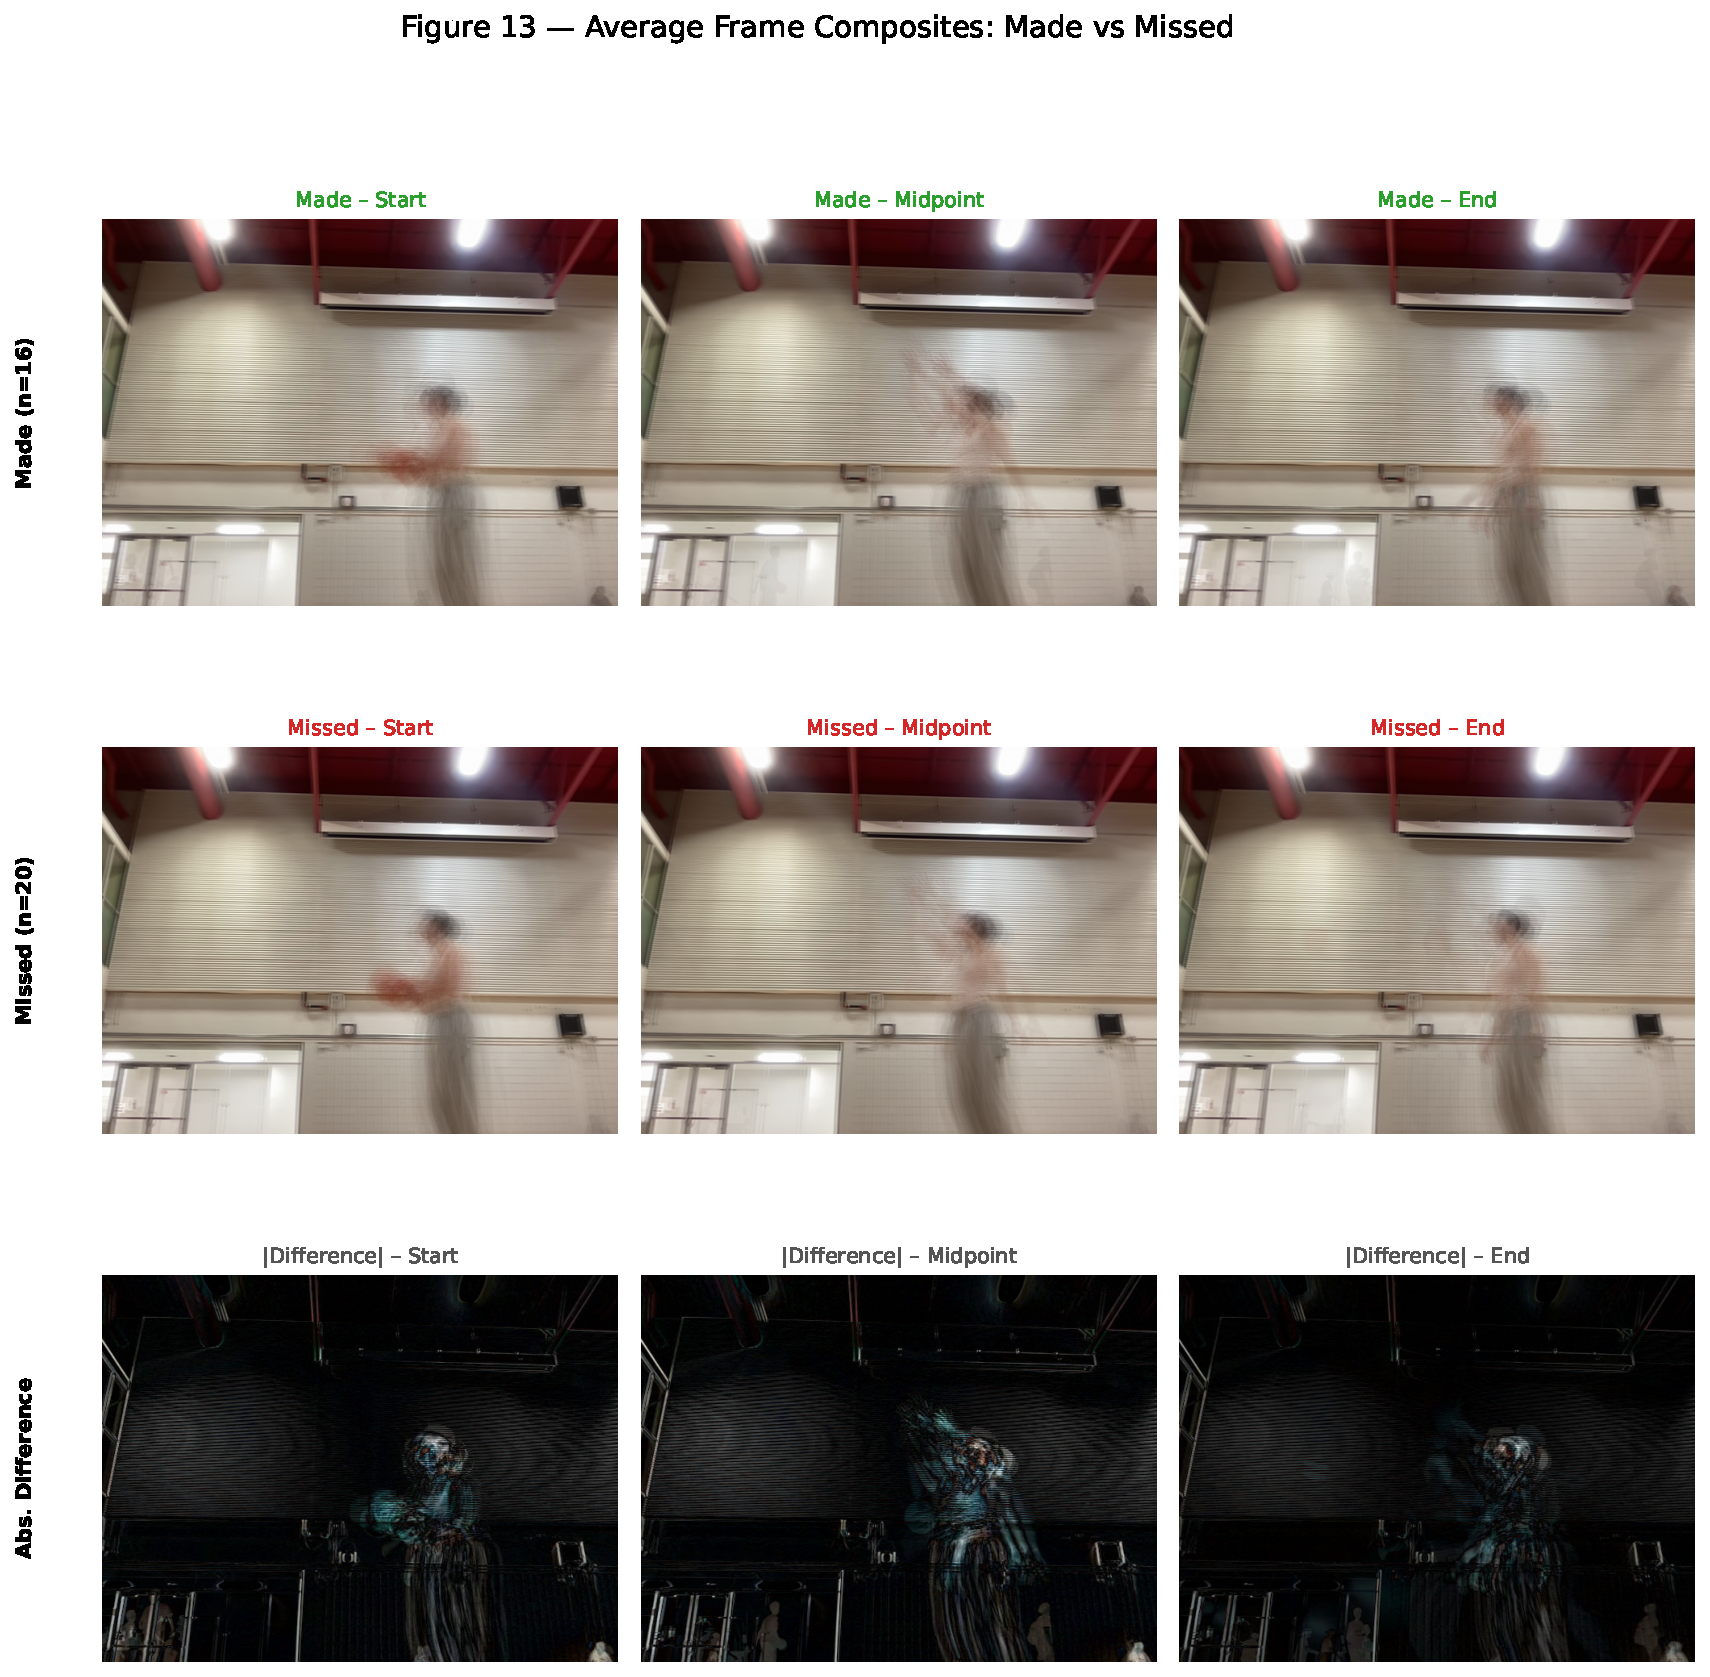
\includegraphics[width=\textwidth]{figures/fig_average_frames.pdf}
  \caption{Average frame composites. Top row: made shots. Middle row: missed
  shots. Bottom row: absolute pixel difference. Columns correspond to
  execution start, midpoint, and end.}
  \label{fig:avgframes}
\end{figure}

% ────────────────────────────────────────────────────────────────────────────
\section{Discussion}

This session (78 analysed shots across 3 blocks, 44\% accuracy) demonstrates that the FreethrowEEG system can capture frequency-band-specific EEG dynamics during free-throw shooting using a portable Muse~2 headset with real EEG data.

Effect sizes for pre-shot band power differences were generally small. With 78 shots across 3 blocks, statistical power remains limited, though substantially improved over the initial pilot.

The $\theta/\alpha$ ratio was higher for made shots, which is broadly consistent with prior literature linking theta/alpha dynamics to attentional focus during precision tasks. Replication with more trials is essential.

The shot-by-shot progression analysis provides a preliminary look at temporal dynamics across the session. Changes in band power over successive shots may reflect fatigue, adaptation, or strategy adjustment, though the current data cannot distinguish between these.

Video-based pose estimation using MediaPipe revealed descriptive differences in shooting kinematics between made and missed shots. Stop-motion decomposition and ghost-overlay composites provide visual evidence of form consistency, while time-aligned pose and EEG traces offer a preliminary window into the brain--body dynamics underlying free-throw execution.

\subsection{Limitations}
This analysis is based on 78 shots across 3 blocks, after
exclusion of trials with data quality issues and experimenter-flagged missed
cues. Block~1's EEG recording terminated early, yielding only 3 usable shots
from that block. Block~2 lacked video, limiting biomechanical analysis to
Block~3 only. The Muse~2 provides only four channels, precluding source
localization or detailed topographic analysis. Band power values represent
averages across all channels, which may obscure hemisphere-specific effects.
The participant noted increasing fatigue across blocks, particularly in
Block~3, which may confound longitudinal comparisons. Future sessions with
multiple participants and counterbalanced block ordering are needed to draw
reliable conclusions.

% ────────────────────────────────────────────────────────────────────────────
\section{Conclusion}

This multi-block session demonstrates that the FreethrowEEG system can
successfully record and analyse EEG band power during free-throw shooting with
a portable Muse headset under real experimental conditions. With 78
valid shots, this represents a substantial step up from the initial 10-shot
pilot, providing more robust estimates of band-power differences between made
and missed shots. Exploratory analyses identified Theta band power as potentially differentiating made from missed shots. The addition of video-based pose
estimation provides a complementary kinematic dimension, enabling time-aligned
analysis of brain and body dynamics during shot execution. Ghost overlays and
average frame composites offer intuitive visual summaries of shooting form
variability. These results provide a foundation for larger-scale data
collection with multiple participants and more rigorous hypothesis testing.

\end{document}
